\documentclass{book}
\usepackage[a4paper,top=2.5cm,bottom=2.5cm,left=2.5cm,right=2.5cm]{geometry}
\usepackage{makeidx}
\usepackage{natbib}
\usepackage{graphicx}
\usepackage{multicol}
\usepackage{float}
\usepackage{listings}
\usepackage{color}
\usepackage{ifthen}
\usepackage[table]{xcolor}
\usepackage{textcomp}
\usepackage{alltt}
\usepackage{ifpdf}
\ifpdf
\usepackage[pdftex,
            pagebackref=true,
            colorlinks=true,
            linkcolor=blue,
            unicode
           ]{hyperref}
\else
\usepackage[ps2pdf,
            pagebackref=true,
            colorlinks=true,
            linkcolor=blue,
            unicode
           ]{hyperref}
\usepackage{pspicture}
\fi
\usepackage[utf8]{inputenc}
\usepackage{mathptmx}
\usepackage[scaled=.90]{helvet}
\usepackage{courier}
\usepackage{sectsty}
\usepackage{amssymb}
\usepackage[titles]{tocloft}
\usepackage{doxygen}
\lstset{language=C++,inputencoding=utf8,basicstyle=\footnotesize,breaklines=true,breakatwhitespace=true,tabsize=4,numbers=left }
\makeindex
\setcounter{tocdepth}{3}
\renewcommand{\footrulewidth}{0.4pt}
\renewcommand{\familydefault}{\sfdefault}
\hfuzz=15pt
\setlength{\emergencystretch}{15pt}
\hbadness=750
\tolerance=750
\begin{document}
\hypersetup{pageanchor=false,citecolor=blue}
\begin{titlepage}
\vspace*{7cm}
\begin{center}
{\Large cpplatex }\\
\vspace*{1cm}
{\large Generated by Doxygen 1.8.3.1}\\
\vspace*{0.5cm}
{\small Tue Nov 1 2016 23:28:09}\\
\end{center}
\end{titlepage}
\clearemptydoublepage
\pagenumbering{roman}
\tableofcontents
\clearemptydoublepage
\pagenumbering{arabic}
\hypersetup{pageanchor=true,citecolor=blue}
\chapter{cpplatex}
\label{md_README}
\hypertarget{md_README}{}
\href{https://travis-ci.org/zmarcantel/cpplatex}{\tt !\mbox{[}Build Status\mbox{]}(https\-://travis-\/ci.\-org/zmarcantel/cpplatex.\-svg?branch=master)}

Header-\/only {\ttfamily La\-Te\-X} document builder in C++14.

An important feature is the ability to do (templated) math operations and get out not only the arithmetic result, but a fully {\ttfamily La\-Te\-X}-\/formatted representation.

This allows the user to do complex/scientific math using external libraries while being able to programmatically generate reports, documentation, etc. from the calculations themselves with almost no effort.

\section*{quick example}

For more in-\/depth examples, see the tests.

```cpp \#include \char`\"{}cpplatex.\-hpp\char`\"{}

...

\#define N\-U\-M(x) latex\-::math\-::make\-\_\-num(x) \#define E\-X\-P(x, y) latex\-::math\-::make\-\_\-exp(x, y) \#define R\-O\-O\-T(x, y) latex\-::math\-::make\-\_\-root(x, y)

static latex\-::math\-::\-Number$<$double$>$ P\-I(3.\-14);

void find\-\_\-area\-\_\-and\-\_\-volume(double height, double radius) \{ auto area = P\-I $\ast$ E\-X\-P(radius, 2); auto volume = P\-I $\ast$ pow(radius, 2) $\ast$ height;

std\-::cout $<$$<$ area $<$$<$ std\-::endl; // output the La\-Te\-X formatted string std\-::cout $<$$<$ area.\-solve() $<$$<$ std\-::endl; // output the area of this base

std\-::cout $<$$<$ volume $<$$<$ std\-::endl; // output the La\-Te\-X formatted string std\-::cout $<$$<$ volume.\-solve() $<$$<$ std\-::endl; // output the volume of this cylinder \}

void complex\-\_\-equation() \{ // (sqrt(\-P\-I $\ast$ 4) + 14.\-68 + log3(10))$^\wedge$4 // -\/-\/-\/-\/-\/-\/-\/-\/-\/-\/-\/-\/-\/-\/-\/-\/-\/-\/-\/-\/-\/-\/-\/-\/-\/-\/-\/-\/-\/-\/-\/-\/--- // cube\-\_\-root(9) auto eqn = ((P\-I $\ast$ 4).sqrt() + 14.\-68 + N\-U\-M(10).log(3)).pow(4) / R\-O\-O\-T(9, 3);

std\-::cout $<$$<$ eqn $<$$<$ std\-::endl; // output the La\-Te\-X formatted string std\-::cout $<$$<$ eqn.\-solve() $<$$<$ std\-::endl; // output the reduced value of this complex equation \}

void make\-\_\-doc() \{ // you can use the builder pattern...

latex\-::doc\-::\-Document$<$latex\-::doc\-::doctypes\-::\-Report$>$ doc(\char`\"{}\-Some Title\char`\"{}, \char`\"{}\-And A Subtitle\char`\"{}); doc.\-with\-\_\-toc() // use a table of contents .use(\char`\"{}some\-\_\-import\char`\"{}) // use the \char`\"{}some\-\_\-import\char`\"{} package .use(\char`\"{}another\-\_\-import\char`\"{}) // use another package .with\-\_\-leading\-\_\-content(\char`\"{}some content to insert\char`\"{}); // add some content before we get to the sections

// ... the streaming pattern

\hyperlink{classlatex_1_1doc_1_1Section}{latex\-::doc\-::\-Section} intro(\char`\"{}\-Introduction\char`\"{}); intro $<$$<$ \char`\"{}\-Blah blah, oh, and blah.\char`\"{};

doc $<$$<$ intro;

// ... or a mix of both! handy dandy.

// print your document

std\-::cout $<$$<$ doc;

// or store it

auto doc\-\_\-str = doc.\-to\-\_\-string();

// or build it into a std\-::ostream

std\-::stringstream ss; doc.\-build(ss); \} ``` 
\chapter{Class Index}
\section{Class List}
Here are the classes, structs, unions and interfaces with brief descriptions\-:\begin{DoxyCompactList}
\item\contentsline{section}{\hyperlink{classlatex_1_1math_1_1Addition}{latex\-::math\-::\-Addition$<$ L\-H\-S, R\-H\-S $>$} }{\pageref{classlatex_1_1math_1_1Addition}}{}
\item\contentsline{section}{\hyperlink{classlatex_1_1math_1_1AlignedEquation}{latex\-::math\-::\-Aligned\-Equation$<$ L\-H\-S, Steps $>$} }{\pageref{classlatex_1_1math_1_1AlignedEquation}}{}
\item\contentsline{section}{\hyperlink{classlatex_1_1doc_1_1doctypes_1_1Article}{latex\-::doc\-::doctypes\-::\-Article} }{\pageref{classlatex_1_1doc_1_1doctypes_1_1Article}}{}
\item\contentsline{section}{\hyperlink{classlatex_1_1style_1_1Bold}{latex\-::style\-::\-Bold} }{\pageref{classlatex_1_1style_1_1Bold}}{}
\item\contentsline{section}{\hyperlink{classlatex_1_1doc_1_1doctypes_1_1Book}{latex\-::doc\-::doctypes\-::\-Book} }{\pageref{classlatex_1_1doc_1_1doctypes_1_1Book}}{}
\item\contentsline{section}{\hyperlink{classlatex_1_1doc_1_1Document}{latex\-::doc\-::\-Document$<$ Doc\-Type, font\-\_\-size $>$} }{\pageref{classlatex_1_1doc_1_1Document}}{}
\item\contentsline{section}{\hyperlink{classlatex_1_1math_1_1Equation}{latex\-::math\-::\-Equation$<$ L\-H\-S, R\-H\-S $>$} }{\pageref{classlatex_1_1math_1_1Equation}}{}
\item\contentsline{section}{\hyperlink{classlatex_1_1math_1_1Exponent}{latex\-::math\-::\-Exponent$<$ L\-H\-S, R\-H\-S $>$} }{\pageref{classlatex_1_1math_1_1Exponent}}{}
\item\contentsline{section}{\hyperlink{classlatex_1_1math_1_1Fraction}{latex\-::math\-::\-Fraction$<$ L\-H\-S, R\-H\-S $>$} }{\pageref{classlatex_1_1math_1_1Fraction}}{}
\item\contentsline{section}{\hyperlink{classlatex_1_1style_1_1Huge}{latex\-::style\-::\-Huge} }{\pageref{classlatex_1_1style_1_1Huge}}{}
\item\contentsline{section}{\hyperlink{classlatex_1_1style_1_1Huger}{latex\-::style\-::\-Huger} }{\pageref{classlatex_1_1style_1_1Huger}}{}
\item\contentsline{section}{\hyperlink{classlatex_1_1style_1_1Italic}{latex\-::style\-::\-Italic} }{\pageref{classlatex_1_1style_1_1Italic}}{}
\item\contentsline{section}{\hyperlink{classlatex_1_1style_1_1Large}{latex\-::style\-::\-Large} }{\pageref{classlatex_1_1style_1_1Large}}{}
\item\contentsline{section}{\hyperlink{classlatex_1_1style_1_1Larger}{latex\-::style\-::\-Larger} }{\pageref{classlatex_1_1style_1_1Larger}}{}
\item\contentsline{section}{\hyperlink{classlatex_1_1style_1_1Largest}{latex\-::style\-::\-Largest} }{\pageref{classlatex_1_1style_1_1Largest}}{}
\item\contentsline{section}{\hyperlink{classlatex_1_1doc_1_1List}{latex\-::doc\-::\-List$<$ Style $>$} }{\pageref{classlatex_1_1doc_1_1List}}{}
\item\contentsline{section}{\hyperlink{classlatex_1_1math_1_1Log}{latex\-::math\-::\-Log$<$ Val, Base $>$} }{\pageref{classlatex_1_1math_1_1Log}}{}
\item\contentsline{section}{\hyperlink{classlatex_1_1math_1_1Multiplication}{latex\-::math\-::\-Multiplication$<$ L\-H\-S, R\-H\-S $>$} }{\pageref{classlatex_1_1math_1_1Multiplication}}{}
\item\contentsline{section}{\hyperlink{classlatex_1_1math_1_1NaturalLog}{latex\-::math\-::\-Natural\-Log$<$ Val $>$} }{\pageref{classlatex_1_1math_1_1NaturalLog}}{}
\item\contentsline{section}{\hyperlink{classlatex_1_1style_1_1None}{latex\-::style\-::\-None} }{\pageref{classlatex_1_1style_1_1None}}{}
\item\contentsline{section}{\hyperlink{classlatex_1_1style_1_1Normal}{latex\-::style\-::\-Normal} }{\pageref{classlatex_1_1style_1_1Normal}}{}
\item\contentsline{section}{\hyperlink{classlatex_1_1math_1_1Number}{latex\-::math\-::\-Number$<$ T $>$} }{\pageref{classlatex_1_1math_1_1Number}}{}
\item\contentsline{section}{\hyperlink{classlatex_1_1doc_1_1listtypes_1_1Ordered}{latex\-::doc\-::listtypes\-::\-Ordered} }{\pageref{classlatex_1_1doc_1_1listtypes_1_1Ordered}}{}
\item\contentsline{section}{\hyperlink{classlatex_1_1math_1_1Paren}{latex\-::math\-::\-Paren$<$ T $>$} }{\pageref{classlatex_1_1math_1_1Paren}}{}
\item\contentsline{section}{\hyperlink{classlatex_1_1doc_1_1doctypes_1_1Report}{latex\-::doc\-::doctypes\-::\-Report} }{\pageref{classlatex_1_1doc_1_1doctypes_1_1Report}}{}
\item\contentsline{section}{\hyperlink{classlatex_1_1math_1_1Root}{latex\-::math\-::\-Root$<$ Val, Power $>$} }{\pageref{classlatex_1_1math_1_1Root}}{}
\item\contentsline{section}{\hyperlink{classlatex_1_1doc_1_1Section}{latex\-::doc\-::\-Section} }{\pageref{classlatex_1_1doc_1_1Section}}{}
\item\contentsline{section}{\hyperlink{classlatex_1_1style_1_1Small}{latex\-::style\-::\-Small} }{\pageref{classlatex_1_1style_1_1Small}}{}
\item\contentsline{section}{\hyperlink{classlatex_1_1math_1_1SubscriptedVariable}{latex\-::math\-::\-Subscripted\-Variable$<$ Upper, Lower $>$} }{\pageref{classlatex_1_1math_1_1SubscriptedVariable}}{}
\item\contentsline{section}{\hyperlink{classlatex_1_1doc_1_1Subsection}{latex\-::doc\-::\-Subsection} }{\pageref{classlatex_1_1doc_1_1Subsection}}{}
\item\contentsline{section}{\hyperlink{classlatex_1_1math_1_1Subtraction}{latex\-::math\-::\-Subtraction$<$ L\-H\-S, R\-H\-S $>$} }{\pageref{classlatex_1_1math_1_1Subtraction}}{}
\item\contentsline{section}{\hyperlink{classlatex_1_1Text}{latex\-::\-Text$<$ Style, Rest $>$} }{\pageref{classlatex_1_1Text}}{}
\item\contentsline{section}{\hyperlink{classlatex_1_1style_1_1Tiny}{latex\-::style\-::\-Tiny} }{\pageref{classlatex_1_1style_1_1Tiny}}{}
\item\contentsline{section}{\hyperlink{classlatex_1_1style_1_1Underline}{latex\-::style\-::\-Underline} }{\pageref{classlatex_1_1style_1_1Underline}}{}
\item\contentsline{section}{\hyperlink{classlatex_1_1doc_1_1listtypes_1_1Unordered}{latex\-::doc\-::listtypes\-::\-Unordered} }{\pageref{classlatex_1_1doc_1_1listtypes_1_1Unordered}}{}
\item\contentsline{section}{\hyperlink{classlatex_1_1math_1_1ValuedVariable}{latex\-::math\-::\-Valued\-Variable$<$ T, Str\-Type $>$} }{\pageref{classlatex_1_1math_1_1ValuedVariable}}{}
\item\contentsline{section}{\hyperlink{classlatex_1_1math_1_1Variable}{latex\-::math\-::\-Variable$<$ T $>$} }{\pageref{classlatex_1_1math_1_1Variable}}{}
\end{DoxyCompactList}

\chapter{Class Documentation}
\hypertarget{classlatex_1_1math_1_1Addition}{\section{latex\-:\-:math\-:\-:Addition$<$ L\-H\-S, R\-H\-S $>$ Class Template Reference}
\label{classlatex_1_1math_1_1Addition}\index{latex\-::math\-::\-Addition$<$ L\-H\-S, R\-H\-S $>$@{latex\-::math\-::\-Addition$<$ L\-H\-S, R\-H\-S $>$}}
}


Inheritance diagram for latex\-:\-:math\-:\-:Addition$<$ L\-H\-S, R\-H\-S $>$\-:
\nopagebreak
\begin{figure}[H]
\begin{center}
\leavevmode
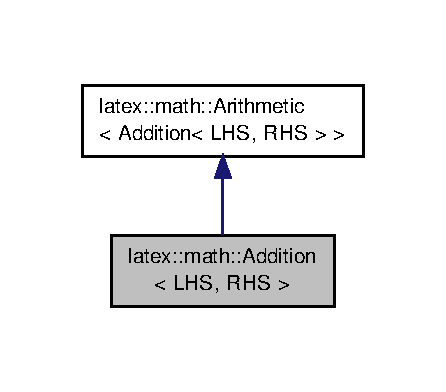
\includegraphics[width=214pt]{classlatex_1_1math_1_1Addition__inherit__graph}
\end{center}
\end{figure}


Collaboration diagram for latex\-:\-:math\-:\-:Addition$<$ L\-H\-S, R\-H\-S $>$\-:
\nopagebreak
\begin{figure}[H]
\begin{center}
\leavevmode
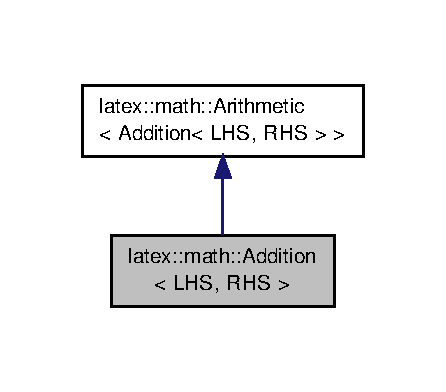
\includegraphics[width=214pt]{classlatex_1_1math_1_1Addition__coll__graph}
\end{center}
\end{figure}
\subsection*{Public Types}
\begin{DoxyCompactItemize}
\item 
\hypertarget{classlatex_1_1math_1_1Addition_aaea872c65a92e8d4b30947abe9908517}{using {\bfseries L\-H\-S\-Type} = L\-H\-S}\label{classlatex_1_1math_1_1Addition_aaea872c65a92e8d4b30947abe9908517}

\item 
\hypertarget{classlatex_1_1math_1_1Addition_a0fe2a62eec58bbfd834b631f06c601c5}{using {\bfseries R\-H\-S\-Type} = R\-H\-S}\label{classlatex_1_1math_1_1Addition_a0fe2a62eec58bbfd834b631f06c601c5}

\item 
\hypertarget{classlatex_1_1math_1_1Addition_ac09b52f17f976ceef97ed19c2777c4a0}{using {\bfseries Self} = \hyperlink{classlatex_1_1math_1_1Addition}{Addition}$<$ L\-H\-S, R\-H\-S $>$}\label{classlatex_1_1math_1_1Addition_ac09b52f17f976ceef97ed19c2777c4a0}

\end{DoxyCompactItemize}
\subsection*{Public Member Functions}
\begin{DoxyCompactItemize}
\item 
\hypertarget{classlatex_1_1math_1_1Addition_ade3a2eff41f8aaef8f77c2b2bb238b57}{{\bfseries Addition} (L\-H\-S lhs, R\-H\-S rhs)}\label{classlatex_1_1math_1_1Addition_ade3a2eff41f8aaef8f77c2b2bb238b57}

\item 
\hypertarget{classlatex_1_1math_1_1Addition_a69f19bb11a63d8631b6e0d246b994c00}{auto {\bfseries solve} ()}\label{classlatex_1_1math_1_1Addition_a69f19bb11a63d8631b6e0d246b994c00}

\item 
\hypertarget{classlatex_1_1math_1_1Addition_a03c226a26292f1203370bedf162731a0}{std\-::string {\bfseries latex} () const }\label{classlatex_1_1math_1_1Addition_a03c226a26292f1203370bedf162731a0}

\item 
\hypertarget{classlatex_1_1math_1_1Addition_aeb8aded4d72c95ac93539860321f2d0b}{{\footnotesize template$<$typename T $>$ }\\\hyperlink{classlatex_1_1math_1_1Exponent}{Exponent}$<$ \hyperlink{classlatex_1_1math_1_1Addition}{Self}, T $>$ {\bfseries pow} (const T \&power)}\label{classlatex_1_1math_1_1Addition_aeb8aded4d72c95ac93539860321f2d0b}

\item 
\hypertarget{classlatex_1_1math_1_1Addition_aeafa689b3df0a4c99396c3f5d12d40a5}{{\footnotesize template$<$typename Base $>$ }\\\hyperlink{classlatex_1_1math_1_1Log}{Log}$<$ \hyperlink{classlatex_1_1math_1_1Addition}{Self}, Base $>$ {\bfseries log} (Base base)}\label{classlatex_1_1math_1_1Addition_aeafa689b3df0a4c99396c3f5d12d40a5}

\item 
\hypertarget{classlatex_1_1math_1_1Addition_adf1963ebf74f64325555149dcefaf30a}{\hyperlink{classlatex_1_1math_1_1NaturalLog}{Natural\-Log}$<$ \hyperlink{classlatex_1_1math_1_1Addition}{Self} $>$ {\bfseries ln} ()}\label{classlatex_1_1math_1_1Addition_adf1963ebf74f64325555149dcefaf30a}

\item 
\hypertarget{classlatex_1_1math_1_1Addition_a8c94bab6a8b94636f0a1215d8690f273}{\hyperlink{classlatex_1_1math_1_1Root}{Root}$<$ \hyperlink{classlatex_1_1math_1_1Addition}{Self}, int $>$ {\bfseries sqrt} ()}\label{classlatex_1_1math_1_1Addition_a8c94bab6a8b94636f0a1215d8690f273}

\end{DoxyCompactItemize}
\subsection*{Protected Attributes}
\begin{DoxyCompactItemize}
\item 
\hypertarget{classlatex_1_1math_1_1Addition_ac8d2192970f9214c489f803756453bf0}{L\-H\-S {\bfseries lhs}}\label{classlatex_1_1math_1_1Addition_ac8d2192970f9214c489f803756453bf0}

\item 
\hypertarget{classlatex_1_1math_1_1Addition_aa5abec9e5629652699b7e34887ec94a6}{R\-H\-S {\bfseries rhs}}\label{classlatex_1_1math_1_1Addition_aa5abec9e5629652699b7e34887ec94a6}

\end{DoxyCompactItemize}
\subsection*{Friends}
\begin{DoxyCompactItemize}
\item 
\hypertarget{classlatex_1_1math_1_1Addition_a4d362127264a2ef4b53edb9c7a983b18}{std\-::ostream \& {\bfseries operator$<$$<$} (std\-::ostream \&os, const \hyperlink{classlatex_1_1math_1_1Addition}{Addition} \&add)}\label{classlatex_1_1math_1_1Addition_a4d362127264a2ef4b53edb9c7a983b18}

\end{DoxyCompactItemize}


The documentation for this class was generated from the following file\-:\begin{DoxyCompactItemize}
\item 
latex.\-hpp\end{DoxyCompactItemize}

\hypertarget{classlatex_1_1math_1_1AlignedEquation}{\section{latex\-:\-:math\-:\-:Aligned\-Equation$<$ L\-H\-S, Steps $>$ Class Template Reference}
\label{classlatex_1_1math_1_1AlignedEquation}\index{latex\-::math\-::\-Aligned\-Equation$<$ L\-H\-S, Steps $>$@{latex\-::math\-::\-Aligned\-Equation$<$ L\-H\-S, Steps $>$}}
}
\subsection*{Public Member Functions}
\begin{DoxyCompactItemize}
\item 
\hypertarget{classlatex_1_1math_1_1AlignedEquation_aaec92b40e78edcfe25b9e02ba8f7067a}{{\bfseries Aligned\-Equation} (const L\-H\-S \&lhs, Steps...\-steps)}\label{classlatex_1_1math_1_1AlignedEquation_aaec92b40e78edcfe25b9e02ba8f7067a}

\item 
\hypertarget{classlatex_1_1math_1_1AlignedEquation_a2d5ac3f300d83f74f04fd3b73a5b123c}{std\-::string {\bfseries latex} () const }\label{classlatex_1_1math_1_1AlignedEquation_a2d5ac3f300d83f74f04fd3b73a5b123c}

\end{DoxyCompactItemize}
\subsection*{Protected Member Functions}
\begin{DoxyCompactItemize}
\item 
\hypertarget{classlatex_1_1math_1_1AlignedEquation_a362cf33e9e59dc607d615d29573c1343}{{\footnotesize template$<$typename First , typename... T$>$ }\\void {\bfseries print\-\_\-steps} (std\-::ostream \&os, First \&f, T...\-rest)}\label{classlatex_1_1math_1_1AlignedEquation_a362cf33e9e59dc607d615d29573c1343}

\item 
\hypertarget{classlatex_1_1math_1_1AlignedEquation_a98b2b263d90b8f67da373b575804a28d}{{\footnotesize template$<$typename First , typename... T$>$ }\\void {\bfseries print\-\_\-steps} (std\-::ostream \&os, First \&f)}\label{classlatex_1_1math_1_1AlignedEquation_a98b2b263d90b8f67da373b575804a28d}

\end{DoxyCompactItemize}
\subsection*{Protected Attributes}
\begin{DoxyCompactItemize}
\item 
\hypertarget{classlatex_1_1math_1_1AlignedEquation_a5d23378f8a75c041181f62d104670fee}{std\-::string {\bfseries eqn}}\label{classlatex_1_1math_1_1AlignedEquation_a5d23378f8a75c041181f62d104670fee}

\end{DoxyCompactItemize}
\subsection*{Static Protected Attributes}
\begin{DoxyCompactItemize}
\item 
\hypertarget{classlatex_1_1math_1_1AlignedEquation_a19c23a2c3f908d8d167969cd88efef72}{constexpr static const char $\ast$ {\bfseries open\-\_\-context} = \char`\"{}\textbackslash{}\textbackslash{}begin\{equation\}\char`\"{}}\label{classlatex_1_1math_1_1AlignedEquation_a19c23a2c3f908d8d167969cd88efef72}

\item 
\hypertarget{classlatex_1_1math_1_1AlignedEquation_a34eb2b78f0667208d92f61be226cf335}{constexpr static const char $\ast$ {\bfseries close\-\_\-context} = \char`\"{}\textbackslash{}\textbackslash{}end\{equation\}\char`\"{}}\label{classlatex_1_1math_1_1AlignedEquation_a34eb2b78f0667208d92f61be226cf335}

\item 
\hypertarget{classlatex_1_1math_1_1AlignedEquation_a664278f69a33046287403d1bdff81327}{constexpr static const char $\ast$ {\bfseries split\-\_\-eq} = \char`\"{} \& = \char`\"{}}\label{classlatex_1_1math_1_1AlignedEquation_a664278f69a33046287403d1bdff81327}

\end{DoxyCompactItemize}
\subsection*{Friends}
\begin{DoxyCompactItemize}
\item 
\hypertarget{classlatex_1_1math_1_1AlignedEquation_a82ee5c4bf9b60a6704901092d287d3c7}{std\-::ostream \& {\bfseries operator$<$$<$} (std\-::ostream \&os, const \hyperlink{classlatex_1_1math_1_1AlignedEquation}{Aligned\-Equation} \&eq)}\label{classlatex_1_1math_1_1AlignedEquation_a82ee5c4bf9b60a6704901092d287d3c7}

\end{DoxyCompactItemize}


The documentation for this class was generated from the following file\-:\begin{DoxyCompactItemize}
\item 
latex.\-hpp\end{DoxyCompactItemize}

\hypertarget{classlatex_1_1doc_1_1doctypes_1_1Article}{\section{latex\-:\-:doc\-:\-:doctypes\-:\-:\-Article \-Class \-Reference}
\label{classlatex_1_1doc_1_1doctypes_1_1Article}\index{latex\-::doc\-::doctypes\-::\-Article@{latex\-::doc\-::doctypes\-::\-Article}}
}


{\ttfamily \#include $<$latex.\-hpp$>$}

\subsection*{\-Static \-Public \-Attributes}
\begin{DoxyCompactItemize}
\item 
\hypertarget{classlatex_1_1doc_1_1doctypes_1_1Article_a13ce4dd5c712f498e99029a8e8dc77b3}{constexpr static const char $\ast$ {\bfseries header} = \char`\"{}article\char`\"{}}\label{classlatex_1_1doc_1_1doctypes_1_1Article_a13ce4dd5c712f498e99029a8e8dc77b3}

\item 
\hypertarget{classlatex_1_1doc_1_1doctypes_1_1Article_ae8a3378f1d947c6300c7a6d8a01e09fc}{constexpr static const bool {\bfseries can\-\_\-toc} = false}\label{classlatex_1_1doc_1_1doctypes_1_1Article_ae8a3378f1d947c6300c7a6d8a01e09fc}

\item 
\hypertarget{classlatex_1_1doc_1_1doctypes_1_1Article_a7dc7e13e28ac8c09d92e367a1c470a27}{constexpr static const bool {\bfseries can\-\_\-subtitle} = false}\label{classlatex_1_1doc_1_1doctypes_1_1Article_a7dc7e13e28ac8c09d92e367a1c470a27}

\end{DoxyCompactItemize}


\subsection{\-Detailed \-Description}
\-Use the 'article' doctype for document generation. 

\-The documentation for this class was generated from the following file\-:\begin{DoxyCompactItemize}
\item 
latex.\-hpp\end{DoxyCompactItemize}

\hypertarget{classlatex_1_1style_1_1Bold}{\section{latex\-:\-:style\-:\-:\-Bold \-Class \-Reference}
\label{classlatex_1_1style_1_1Bold}\index{latex\-::style\-::\-Bold@{latex\-::style\-::\-Bold}}
}
\subsection*{\-Static \-Public \-Attributes}
\begin{DoxyCompactItemize}
\item 
\hypertarget{classlatex_1_1style_1_1Bold_a3802de3a45ede8381489dc53c647fb82}{constexpr static const char $\ast$ {\bfseries open} = \char`\"{}$\backslash$$\backslash$textbf\{\char`\"{}}\label{classlatex_1_1style_1_1Bold_a3802de3a45ede8381489dc53c647fb82}

\item 
\hypertarget{classlatex_1_1style_1_1Bold_ad81c547be1c60043179f03e24802a64c}{constexpr static const char $\ast$ {\bfseries close} = \char`\"{}\}\char`\"{}}\label{classlatex_1_1style_1_1Bold_ad81c547be1c60043179f03e24802a64c}

\end{DoxyCompactItemize}


\-The documentation for this class was generated from the following file\-:\begin{DoxyCompactItemize}
\item 
latex.\-hpp\end{DoxyCompactItemize}

\hypertarget{classlatex_1_1math_1_1style_1_1Bold}{\section{latex\-:\-:math\-:\-:style\-:\-:Bold Class Reference}
\label{classlatex_1_1math_1_1style_1_1Bold}\index{latex\-::math\-::style\-::\-Bold@{latex\-::math\-::style\-::\-Bold}}
}
\subsection*{Static Public Attributes}
\begin{DoxyCompactItemize}
\item 
\hypertarget{classlatex_1_1math_1_1style_1_1Bold_a1950a427f6a370117c8dc675bd9541da}{constexpr static const char $\ast$ {\bfseries open} = \char`\"{}\textbackslash{}\textbackslash{}boldsymbol\{\char`\"{}}\label{classlatex_1_1math_1_1style_1_1Bold_a1950a427f6a370117c8dc675bd9541da}

\item 
\hypertarget{classlatex_1_1math_1_1style_1_1Bold_adeb97deb8b2dd178a6fcb40ef914e871}{constexpr static const char $\ast$ {\bfseries close} = \char`\"{}\}\char`\"{}}\label{classlatex_1_1math_1_1style_1_1Bold_adeb97deb8b2dd178a6fcb40ef914e871}

\end{DoxyCompactItemize}


The documentation for this class was generated from the following file\-:\begin{DoxyCompactItemize}
\item 
latex.\-hpp\end{DoxyCompactItemize}

\hypertarget{classlatex_1_1doc_1_1doctypes_1_1Book}{\section{latex\-:\-:doc\-:\-:doctypes\-:\-:Book Class Reference}
\label{classlatex_1_1doc_1_1doctypes_1_1Book}\index{latex\-::doc\-::doctypes\-::\-Book@{latex\-::doc\-::doctypes\-::\-Book}}
}


{\ttfamily \#include $<$latex.\-hpp$>$}

\subsection*{Static Public Attributes}
\begin{DoxyCompactItemize}
\item 
\hypertarget{classlatex_1_1doc_1_1doctypes_1_1Book_a36a8b56c9502dab4a4301b1153851540}{constexpr static const char $\ast$ {\bfseries header} = \char`\"{}book\char`\"{}}\label{classlatex_1_1doc_1_1doctypes_1_1Book_a36a8b56c9502dab4a4301b1153851540}

\item 
\hypertarget{classlatex_1_1doc_1_1doctypes_1_1Book_ac71f7b7b881db6ae5b9fa295b02b30f0}{constexpr static const bool {\bfseries can\-\_\-toc} = true}\label{classlatex_1_1doc_1_1doctypes_1_1Book_ac71f7b7b881db6ae5b9fa295b02b30f0}

\item 
\hypertarget{classlatex_1_1doc_1_1doctypes_1_1Book_a07a5af234d52ca56082d3a7d58af5615}{constexpr static const bool {\bfseries can\-\_\-subtitle} = true}\label{classlatex_1_1doc_1_1doctypes_1_1Book_a07a5af234d52ca56082d3a7d58af5615}

\end{DoxyCompactItemize}


\subsection{Detailed Description}
Use the 'book' doctype for document generation. 

The documentation for this class was generated from the following file\-:\begin{DoxyCompactItemize}
\item 
latex.\-hpp\end{DoxyCompactItemize}

\hypertarget{classlatex_1_1math_1_1Cos}{\section{latex\-:\-:math\-:\-:Cos$<$ Val $>$ Class Template Reference}
\label{classlatex_1_1math_1_1Cos}\index{latex\-::math\-::\-Cos$<$ Val $>$@{latex\-::math\-::\-Cos$<$ Val $>$}}
}
\subsection*{Public Types}
\begin{DoxyCompactItemize}
\item 
\hypertarget{classlatex_1_1math_1_1Cos_a154c39b3e1e020d6e6c9b220946a9203}{using {\bfseries Val\-Type} = Val}\label{classlatex_1_1math_1_1Cos_a154c39b3e1e020d6e6c9b220946a9203}

\item 
\hypertarget{classlatex_1_1math_1_1Cos_a2905a73f1686f7b2e111805fe9e53a8a}{using {\bfseries Self} = \hyperlink{classlatex_1_1math_1_1Cos}{Cos}$<$ Val $>$}\label{classlatex_1_1math_1_1Cos_a2905a73f1686f7b2e111805fe9e53a8a}

\end{DoxyCompactItemize}
\subsection*{Public Member Functions}
\begin{DoxyCompactItemize}
\item 
\hypertarget{classlatex_1_1math_1_1Cos_a00d8238b1b96698e137d285e746e5bd0}{{\bfseries Cos} (Val val)}\label{classlatex_1_1math_1_1Cos_a00d8238b1b96698e137d285e746e5bd0}

\item 
\hypertarget{classlatex_1_1math_1_1Cos_abdbafc7009e9be6ce738052aafd109f9}{auto {\bfseries solve} ()}\label{classlatex_1_1math_1_1Cos_abdbafc7009e9be6ce738052aafd109f9}

\item 
\hypertarget{classlatex_1_1math_1_1Cos_a09706240be9ca5a03af56bd4e6ee5db8}{std\-::string {\bfseries latex} () const }\label{classlatex_1_1math_1_1Cos_a09706240be9ca5a03af56bd4e6ee5db8}

\item 
\hypertarget{classlatex_1_1math_1_1Cos_a762f1a56defbf20c544756a5cefef40e}{{\footnotesize template$<$typename T $>$ }\\\hyperlink{classlatex_1_1math_1_1Power}{Power}$<$ \hyperlink{classlatex_1_1math_1_1Cos}{Self}, T $>$ {\bfseries pow} (const T \&power)}\label{classlatex_1_1math_1_1Cos_a762f1a56defbf20c544756a5cefef40e}

\item 
\hypertarget{classlatex_1_1math_1_1Cos_a9234d42396d1a761ed41289215431b78}{{\footnotesize template$<$typename Base $>$ }\\\hyperlink{classlatex_1_1math_1_1Log}{Log}$<$ \hyperlink{classlatex_1_1math_1_1Cos}{Self}, Base $>$ {\bfseries log} (Base base)}\label{classlatex_1_1math_1_1Cos_a9234d42396d1a761ed41289215431b78}

\item 
\hypertarget{classlatex_1_1math_1_1Cos_a94359c6ef1a1c525f3b4729c6f7cb665}{\hyperlink{classlatex_1_1math_1_1NaturalLog}{Natural\-Log}$<$ \hyperlink{classlatex_1_1math_1_1Cos}{Self} $>$ {\bfseries ln} ()}\label{classlatex_1_1math_1_1Cos_a94359c6ef1a1c525f3b4729c6f7cb665}

\item 
\hypertarget{classlatex_1_1math_1_1Cos_afc496ab4e4d007e52b74e3cf87fe4b4f}{\hyperlink{classlatex_1_1math_1_1Root}{Root}$<$ \hyperlink{classlatex_1_1math_1_1Cos}{Self}, int $>$ {\bfseries sqrt} ()}\label{classlatex_1_1math_1_1Cos_afc496ab4e4d007e52b74e3cf87fe4b4f}

\end{DoxyCompactItemize}
\subsection*{Protected Attributes}
\begin{DoxyCompactItemize}
\item 
\hypertarget{classlatex_1_1math_1_1Cos_ad42d34196872805774e97b29e69a1896}{Val {\bfseries val}}\label{classlatex_1_1math_1_1Cos_ad42d34196872805774e97b29e69a1896}

\end{DoxyCompactItemize}
\subsection*{Friends}
\begin{DoxyCompactItemize}
\item 
\hypertarget{classlatex_1_1math_1_1Cos_ad5ef89e28352b35eb2cae598810a335d}{std\-::ostream \& {\bfseries operator$<$$<$} (std\-::ostream \&os, const \hyperlink{classlatex_1_1math_1_1Cos}{Cos} \&s)}\label{classlatex_1_1math_1_1Cos_ad5ef89e28352b35eb2cae598810a335d}

\end{DoxyCompactItemize}


The documentation for this class was generated from the following file\-:\begin{DoxyCompactItemize}
\item 
latex.\-hpp\end{DoxyCompactItemize}

\hypertarget{classlatex_1_1doc_1_1Document}{\section{latex\-:\-:doc\-:\-:Document$<$ Doc\-Type $>$ Class Template Reference}
\label{classlatex_1_1doc_1_1Document}\index{latex\-::doc\-::\-Document$<$ Doc\-Type $>$@{latex\-::doc\-::\-Document$<$ Doc\-Type $>$}}
}


{\ttfamily \#include $<$latex.\-hpp$>$}

\subsection*{Public Member Functions}
\begin{DoxyCompactItemize}
\item 
\hypertarget{classlatex_1_1doc_1_1Document_ad03fa7f0d3271370006d20515a3fd5e0}{{\bfseries Document} (const std\-::string \&title)}\label{classlatex_1_1doc_1_1Document_ad03fa7f0d3271370006d20515a3fd5e0}

\item 
\hypertarget{classlatex_1_1doc_1_1Document_a95756c45b9f7b684d81920832971e6c1}{{\bfseries Document} (const std\-::string \&title, const std\-::string \&subtitle)}\label{classlatex_1_1doc_1_1Document_a95756c45b9f7b684d81920832971e6c1}

\item 
\hyperlink{classlatex_1_1doc_1_1Document}{Document} \& \hyperlink{classlatex_1_1doc_1_1Document_a0f449ee90309de24177f4bbc51bcc404}{use} (const std\-::string \&import)
\item 
\hyperlink{classlatex_1_1doc_1_1Document}{Document} \& \hyperlink{classlatex_1_1doc_1_1Document_a02070e69275d800b16c25f99725b5363}{with\-\_\-leading\-\_\-content} (const std\-::string \&content)
\item 
\hyperlink{classlatex_1_1doc_1_1Document}{Document} \& \hyperlink{classlatex_1_1doc_1_1Document_a42eea3ed819c215c5addf8b10fae4302}{with\-\_\-toc} ()
\item 
void \hyperlink{classlatex_1_1doc_1_1Document_a4225432b9f4e3837c4251c9b97c413c6}{write\-\_\-leading} (const std\-::string \&content)
\item 
\hypertarget{classlatex_1_1doc_1_1Document_a5a00cc1883a91126f7c9779d1c0990db}{void {\bfseries insert} (const \hyperlink{classlatex_1_1doc_1_1Section}{Section} \&sect)}\label{classlatex_1_1doc_1_1Document_a5a00cc1883a91126f7c9779d1c0990db}

\item 
\hypertarget{classlatex_1_1doc_1_1Document_a86621b9927d388202c62be1a72fcdb42}{\hyperlink{classlatex_1_1doc_1_1Document}{Document} \& {\bfseries operator$<$$<$} (const char $\ast$val)}\label{classlatex_1_1doc_1_1Document_a86621b9927d388202c62be1a72fcdb42}

\item 
\hypertarget{classlatex_1_1doc_1_1Document_a3bfae6320f6798f236e9d1775ab4a987}{\hyperlink{classlatex_1_1doc_1_1Document}{Document} \& {\bfseries operator$<$$<$} (const std\-::string \&val)}\label{classlatex_1_1doc_1_1Document_a3bfae6320f6798f236e9d1775ab4a987}

\item 
\hypertarget{classlatex_1_1doc_1_1Document_a0d011c1af57eea8b68e5aae4ed546d99}{\hyperlink{classlatex_1_1doc_1_1Document}{Document} \& {\bfseries operator$<$$<$} (const \hyperlink{classlatex_1_1doc_1_1Section}{Section} \&val)}\label{classlatex_1_1doc_1_1Document_a0d011c1af57eea8b68e5aae4ed546d99}

\item 
std\-::string \hyperlink{classlatex_1_1doc_1_1Document_ad62f7f8b1f05f3d6edb2734ba0611913}{to\-\_\-string} () const 
\item 
void \hyperlink{classlatex_1_1doc_1_1Document_a8ae50f6e90452fce2dc036b8fd30a052}{build} (std\-::ostream \&ss) const 
\end{DoxyCompactItemize}
\subsection*{Public Attributes}
\begin{DoxyCompactItemize}
\item 
\hypertarget{classlatex_1_1doc_1_1Document_ae669c421fa782997eae2aed024d7fc53}{std\-::string {\bfseries title}}\label{classlatex_1_1doc_1_1Document_ae669c421fa782997eae2aed024d7fc53}

\item 
\hypertarget{classlatex_1_1doc_1_1Document_a966c4725ea244d9ac8a40335202cb499}{std\-::string {\bfseries subtitle}}\label{classlatex_1_1doc_1_1Document_a966c4725ea244d9ac8a40335202cb499}

\item 
\hypertarget{classlatex_1_1doc_1_1Document_ab7d78e94c5883a7e7adcfa141039d128}{bool {\bfseries use\-\_\-toc}}\label{classlatex_1_1doc_1_1Document_ab7d78e94c5883a7e7adcfa141039d128}

\item 
\hypertarget{classlatex_1_1doc_1_1Document_aa6f47f638c00b57aaed3fca96a7eeab8}{std\-::vector$<$ std\-::string $>$ {\bfseries imports}}\label{classlatex_1_1doc_1_1Document_aa6f47f638c00b57aaed3fca96a7eeab8}

\item 
\hypertarget{classlatex_1_1doc_1_1Document_a69c709a155dcf20df20a353b0d2ec245}{std\-::vector$<$ std\-::string $>$ {\bfseries leading\-\_\-contents}}\label{classlatex_1_1doc_1_1Document_a69c709a155dcf20df20a353b0d2ec245}

\item 
\hypertarget{classlatex_1_1doc_1_1Document_a504d1c3f8c3d3492a13bfb0c249f699f}{std\-::vector$<$ \hyperlink{classlatex_1_1doc_1_1Section}{Section} $>$ {\bfseries sections}}\label{classlatex_1_1doc_1_1Document_a504d1c3f8c3d3492a13bfb0c249f699f}

\end{DoxyCompactItemize}
\subsection*{Friends}
\begin{DoxyCompactItemize}
\item 
\hypertarget{classlatex_1_1doc_1_1Document_a278308e5ad27667f48b2daf57dd1b254}{std\-::ostream \& {\bfseries operator$<$$<$} (std\-::ostream \&os, const \hyperlink{classlatex_1_1doc_1_1Document}{Document} \&doc)}\label{classlatex_1_1doc_1_1Document_a278308e5ad27667f48b2daf57dd1b254}

\end{DoxyCompactItemize}


\subsection{Detailed Description}
\subsubsection*{template$<$typename Doc\-Type = doctypes\-::\-Article$>$class latex\-::doc\-::\-Document$<$ Doc\-Type $>$}

Defines a document which is the root for generating a valid La\-Te\-X document.

Documents must be given a title, and optionally a subtitle.

If the document type supports a table of contents, one is generated after the title page. Table of contents can be toggled via the {\ttfamily \-::use\-\_\-toc} variable or {\ttfamily \-::with\-\_\-toc()} function.

The {\ttfamily \-::use()} function allows importing La\-Te\-X packages.

Leading content is output first, followed by all sections (and their subsections). 

\subsection{Member Function Documentation}
\hypertarget{classlatex_1_1doc_1_1Document_a8ae50f6e90452fce2dc036b8fd30a052}{\index{latex\-::doc\-::\-Document@{latex\-::doc\-::\-Document}!build@{build}}
\index{build@{build}!latex::doc::Document@{latex\-::doc\-::\-Document}}
\subsubsection[{build}]{\setlength{\rightskip}{0pt plus 5cm}template$<$typename Doc\-Type  = doctypes\-::\-Article$>$ void {\bf latex\-::doc\-::\-Document}$<$ Doc\-Type $>$\-::build (
\begin{DoxyParamCaption}
\item[{std\-::ostream \&}]{ss}
\end{DoxyParamCaption}
) const\hspace{0.3cm}{\ttfamily [inline]}}}\label{classlatex_1_1doc_1_1Document_a8ae50f6e90452fce2dc036b8fd30a052}
Helper for outputting the document to a generic std\-::ostream \hypertarget{classlatex_1_1doc_1_1Document_ad62f7f8b1f05f3d6edb2734ba0611913}{\index{latex\-::doc\-::\-Document@{latex\-::doc\-::\-Document}!to\-\_\-string@{to\-\_\-string}}
\index{to\-\_\-string@{to\-\_\-string}!latex::doc::Document@{latex\-::doc\-::\-Document}}
\subsubsection[{to\-\_\-string}]{\setlength{\rightskip}{0pt plus 5cm}template$<$typename Doc\-Type  = doctypes\-::\-Article$>$ std\-::string {\bf latex\-::doc\-::\-Document}$<$ Doc\-Type $>$\-::to\-\_\-string (
\begin{DoxyParamCaption}
{}
\end{DoxyParamCaption}
) const\hspace{0.3cm}{\ttfamily [inline]}}}\label{classlatex_1_1doc_1_1Document_ad62f7f8b1f05f3d6edb2734ba0611913}
Get the entire, La\-Te\-X-\/formatted, document in a std\-::string. \hypertarget{classlatex_1_1doc_1_1Document_a0f449ee90309de24177f4bbc51bcc404}{\index{latex\-::doc\-::\-Document@{latex\-::doc\-::\-Document}!use@{use}}
\index{use@{use}!latex::doc::Document@{latex\-::doc\-::\-Document}}
\subsubsection[{use}]{\setlength{\rightskip}{0pt plus 5cm}template$<$typename Doc\-Type  = doctypes\-::\-Article$>$ {\bf Document}\& {\bf latex\-::doc\-::\-Document}$<$ Doc\-Type $>$\-::use (
\begin{DoxyParamCaption}
\item[{const std\-::string \&}]{import}
\end{DoxyParamCaption}
)\hspace{0.3cm}{\ttfamily [inline]}}}\label{classlatex_1_1doc_1_1Document_a0f449ee90309de24177f4bbc51bcc404}
Import a package into the document \hypertarget{classlatex_1_1doc_1_1Document_a02070e69275d800b16c25f99725b5363}{\index{latex\-::doc\-::\-Document@{latex\-::doc\-::\-Document}!with\-\_\-leading\-\_\-content@{with\-\_\-leading\-\_\-content}}
\index{with\-\_\-leading\-\_\-content@{with\-\_\-leading\-\_\-content}!latex::doc::Document@{latex\-::doc\-::\-Document}}
\subsubsection[{with\-\_\-leading\-\_\-content}]{\setlength{\rightskip}{0pt plus 5cm}template$<$typename Doc\-Type  = doctypes\-::\-Article$>$ {\bf Document}\& {\bf latex\-::doc\-::\-Document}$<$ Doc\-Type $>$\-::with\-\_\-leading\-\_\-content (
\begin{DoxyParamCaption}
\item[{const std\-::string \&}]{content}
\end{DoxyParamCaption}
)\hspace{0.3cm}{\ttfamily [inline]}}}\label{classlatex_1_1doc_1_1Document_a02070e69275d800b16c25f99725b5363}
Builder pattern method for adding leading content \hypertarget{classlatex_1_1doc_1_1Document_a42eea3ed819c215c5addf8b10fae4302}{\index{latex\-::doc\-::\-Document@{latex\-::doc\-::\-Document}!with\-\_\-toc@{with\-\_\-toc}}
\index{with\-\_\-toc@{with\-\_\-toc}!latex::doc::Document@{latex\-::doc\-::\-Document}}
\subsubsection[{with\-\_\-toc}]{\setlength{\rightskip}{0pt plus 5cm}template$<$typename Doc\-Type  = doctypes\-::\-Article$>$ {\bf Document}\& {\bf latex\-::doc\-::\-Document}$<$ Doc\-Type $>$\-::with\-\_\-toc (
\begin{DoxyParamCaption}
{}
\end{DoxyParamCaption}
)\hspace{0.3cm}{\ttfamily [inline]}}}\label{classlatex_1_1doc_1_1Document_a42eea3ed819c215c5addf8b10fae4302}
Enable the table of contents if allowed by the document type \hypertarget{classlatex_1_1doc_1_1Document_a4225432b9f4e3837c4251c9b97c413c6}{\index{latex\-::doc\-::\-Document@{latex\-::doc\-::\-Document}!write\-\_\-leading@{write\-\_\-leading}}
\index{write\-\_\-leading@{write\-\_\-leading}!latex::doc::Document@{latex\-::doc\-::\-Document}}
\subsubsection[{write\-\_\-leading}]{\setlength{\rightskip}{0pt plus 5cm}template$<$typename Doc\-Type  = doctypes\-::\-Article$>$ void {\bf latex\-::doc\-::\-Document}$<$ Doc\-Type $>$\-::write\-\_\-leading (
\begin{DoxyParamCaption}
\item[{const std\-::string \&}]{content}
\end{DoxyParamCaption}
)\hspace{0.3cm}{\ttfamily [inline]}}}\label{classlatex_1_1doc_1_1Document_a4225432b9f4e3837c4251c9b97c413c6}
Write leading text (what comes before the sections in the document) into the document. 

The documentation for this class was generated from the following file\-:\begin{DoxyCompactItemize}
\item 
latex.\-hpp\end{DoxyCompactItemize}

\hypertarget{classlatex_1_1math_1_1Equation}{\section{latex\-:\-:math\-:\-:Equation$<$ L\-H\-S, R\-H\-S $>$ Class Template Reference}
\label{classlatex_1_1math_1_1Equation}\index{latex\-::math\-::\-Equation$<$ L\-H\-S, R\-H\-S $>$@{latex\-::math\-::\-Equation$<$ L\-H\-S, R\-H\-S $>$}}
}
\subsection*{Public Types}
\begin{DoxyCompactItemize}
\item 
\hypertarget{classlatex_1_1math_1_1Equation_aa9edc347823879f6651a4b3dbe31060f}{using {\bfseries L\-H\-S\-Type} = L\-H\-S}\label{classlatex_1_1math_1_1Equation_aa9edc347823879f6651a4b3dbe31060f}

\item 
\hypertarget{classlatex_1_1math_1_1Equation_a70e604aaab38b87af4df46932fab25cc}{using {\bfseries R\-H\-S\-Type} = R\-H\-S}\label{classlatex_1_1math_1_1Equation_a70e604aaab38b87af4df46932fab25cc}

\end{DoxyCompactItemize}
\subsection*{Public Member Functions}
\begin{DoxyCompactItemize}
\item 
\hypertarget{classlatex_1_1math_1_1Equation_abf2df112f6302c99b56fa31927142d33}{{\bfseries Equation} (L\-H\-S lhs, R\-H\-S rhs)}\label{classlatex_1_1math_1_1Equation_abf2df112f6302c99b56fa31927142d33}

\item 
\hypertarget{classlatex_1_1math_1_1Equation_a354a3d509dd259c1c0b51ab915867169}{{\bfseries Equation} (const std\-::string \&label, L\-H\-S lhs, R\-H\-S rhs)}\label{classlatex_1_1math_1_1Equation_a354a3d509dd259c1c0b51ab915867169}

\item 
\hypertarget{classlatex_1_1math_1_1Equation_a8c74a11c75dee6f3ab7f92a322942704}{void {\bfseries insert\-\_\-label} (std\-::ostream \&os) const }\label{classlatex_1_1math_1_1Equation_a8c74a11c75dee6f3ab7f92a322942704}

\item 
auto \hyperlink{classlatex_1_1math_1_1Equation_a07edd6119b4c578f0bd109501284120b}{solve} ()
\item 
\hypertarget{classlatex_1_1math_1_1Equation_acc052b3d3d93f32438ada7338b641d6e}{std\-::string {\bfseries latex} () const }\label{classlatex_1_1math_1_1Equation_acc052b3d3d93f32438ada7338b641d6e}

\end{DoxyCompactItemize}
\subsection*{Protected Attributes}
\begin{DoxyCompactItemize}
\item 
\hypertarget{classlatex_1_1math_1_1Equation_a8e2395207a86cc6fda70df7e31ca004f}{L\-H\-S {\bfseries lhs}}\label{classlatex_1_1math_1_1Equation_a8e2395207a86cc6fda70df7e31ca004f}

\item 
\hypertarget{classlatex_1_1math_1_1Equation_aacaf6103dff8138d0e6836def99dea50}{R\-H\-S {\bfseries rhs}}\label{classlatex_1_1math_1_1Equation_aacaf6103dff8138d0e6836def99dea50}

\item 
\hypertarget{classlatex_1_1math_1_1Equation_af90f3dae754e6f4dbd5e44c0e45a14f5}{std\-::string {\bfseries label}}\label{classlatex_1_1math_1_1Equation_af90f3dae754e6f4dbd5e44c0e45a14f5}

\end{DoxyCompactItemize}
\subsection*{Static Protected Attributes}
\begin{DoxyCompactItemize}
\item 
\hypertarget{classlatex_1_1math_1_1Equation_a9e5c1cbd1b860d6ceff91858cf5f25f1}{constexpr static const char $\ast$ {\bfseries open\-\_\-context} = \char`\"{}\textbackslash{}\textbackslash{}begin\{equation\}\char`\"{}}\label{classlatex_1_1math_1_1Equation_a9e5c1cbd1b860d6ceff91858cf5f25f1}

\item 
\hypertarget{classlatex_1_1math_1_1Equation_aea651eda97f201333c0089cd15e5a339}{constexpr static const char $\ast$ {\bfseries close\-\_\-context} = \char`\"{}\textbackslash{}\textbackslash{}end\{equation\}\char`\"{}}\label{classlatex_1_1math_1_1Equation_aea651eda97f201333c0089cd15e5a339}

\end{DoxyCompactItemize}
\subsection*{Friends}
\begin{DoxyCompactItemize}
\item 
\hypertarget{classlatex_1_1math_1_1Equation_af5648da26fb4c842581cc55ebd721494}{std\-::ostream \& {\bfseries operator$<$$<$} (std\-::ostream \&os, const \hyperlink{classlatex_1_1math_1_1Equation}{Equation} \&eq)}\label{classlatex_1_1math_1_1Equation_af5648da26fb4c842581cc55ebd721494}

\end{DoxyCompactItemize}


\subsection{Member Function Documentation}
\hypertarget{classlatex_1_1math_1_1Equation_a07edd6119b4c578f0bd109501284120b}{\index{latex\-::math\-::\-Equation@{latex\-::math\-::\-Equation}!solve@{solve}}
\index{solve@{solve}!latex::math::Equation@{latex\-::math\-::\-Equation}}
\subsubsection[{solve}]{\setlength{\rightskip}{0pt plus 5cm}template$<$typename L\-H\-S , typename R\-H\-S $>$ auto {\bf latex\-::math\-::\-Equation}$<$ L\-H\-S, R\-H\-S $>$\-::solve (
\begin{DoxyParamCaption}
{}
\end{DoxyParamCaption}
)\hspace{0.3cm}{\ttfamily [inline]}}}\label{classlatex_1_1math_1_1Equation_a07edd6119b4c578f0bd109501284120b}
This {\bfseries does not} solve for variables or balance and solve equations.

It simply reduces the right hand side. 

The documentation for this class was generated from the following file\-:\begin{DoxyCompactItemize}
\item 
latex.\-hpp\end{DoxyCompactItemize}

\hypertarget{classlatex_1_1math_1_1Exponent}{\section{latex\-:\-:math\-:\-:Exponent$<$ R\-H\-S $>$ Class Template Reference}
\label{classlatex_1_1math_1_1Exponent}\index{latex\-::math\-::\-Exponent$<$ R\-H\-S $>$@{latex\-::math\-::\-Exponent$<$ R\-H\-S $>$}}
}
\subsection*{Public Types}
\begin{DoxyCompactItemize}
\item 
\hypertarget{classlatex_1_1math_1_1Exponent_ab88660fc9cebd03743815a5f44555496}{using {\bfseries R\-H\-S\-Type} = R\-H\-S}\label{classlatex_1_1math_1_1Exponent_ab88660fc9cebd03743815a5f44555496}

\item 
\hypertarget{classlatex_1_1math_1_1Exponent_a7ed7d60d3934f7c42fc962c201fa12ae}{using {\bfseries Self} = \hyperlink{classlatex_1_1math_1_1Exponent}{Exponent}$<$ R\-H\-S $>$}\label{classlatex_1_1math_1_1Exponent_a7ed7d60d3934f7c42fc962c201fa12ae}

\end{DoxyCompactItemize}
\subsection*{Public Member Functions}
\begin{DoxyCompactItemize}
\item 
\hypertarget{classlatex_1_1math_1_1Exponent_ab8293dec900c3e88a172436bbafb16d4}{{\bfseries Exponent} (R\-H\-S rhs)}\label{classlatex_1_1math_1_1Exponent_ab8293dec900c3e88a172436bbafb16d4}

\item 
\hypertarget{classlatex_1_1math_1_1Exponent_ac6bc11900331049296afd1cf190ab759}{auto {\bfseries solve} ()}\label{classlatex_1_1math_1_1Exponent_ac6bc11900331049296afd1cf190ab759}

\item 
\hypertarget{classlatex_1_1math_1_1Exponent_a6db4173ded8207b9b77049c594eb49dc}{std\-::string {\bfseries latex} () const }\label{classlatex_1_1math_1_1Exponent_a6db4173ded8207b9b77049c594eb49dc}

\item 
\hypertarget{classlatex_1_1math_1_1Exponent_a8220d1ffafdf8eeefd502488fa91606f}{{\footnotesize template$<$typename T $>$ }\\\hyperlink{classlatex_1_1math_1_1Power}{Power}$<$ \hyperlink{classlatex_1_1math_1_1Exponent}{Self}, T $>$ {\bfseries pow} (const T \&power)}\label{classlatex_1_1math_1_1Exponent_a8220d1ffafdf8eeefd502488fa91606f}

\item 
\hypertarget{classlatex_1_1math_1_1Exponent_ac68c345fbf1a3dcd6cf58673e052ebd9}{{\footnotesize template$<$typename Base $>$ }\\\hyperlink{classlatex_1_1math_1_1Log}{Log}$<$ \hyperlink{classlatex_1_1math_1_1Exponent}{Self}, Base $>$ {\bfseries log} (Base base)}\label{classlatex_1_1math_1_1Exponent_ac68c345fbf1a3dcd6cf58673e052ebd9}

\item 
\hypertarget{classlatex_1_1math_1_1Exponent_ac91297ba0e04c868e27b22e19db84002}{\hyperlink{classlatex_1_1math_1_1NaturalLog}{Natural\-Log}$<$ \hyperlink{classlatex_1_1math_1_1Exponent}{Self} $>$ {\bfseries ln} ()}\label{classlatex_1_1math_1_1Exponent_ac91297ba0e04c868e27b22e19db84002}

\item 
\hypertarget{classlatex_1_1math_1_1Exponent_a06e7e698f6747c1a38a80e0ecf5bee0b}{\hyperlink{classlatex_1_1math_1_1Root}{Root}$<$ \hyperlink{classlatex_1_1math_1_1Exponent}{Self}, int $>$ {\bfseries sqrt} ()}\label{classlatex_1_1math_1_1Exponent_a06e7e698f6747c1a38a80e0ecf5bee0b}

\end{DoxyCompactItemize}
\subsection*{Protected Attributes}
\begin{DoxyCompactItemize}
\item 
\hypertarget{classlatex_1_1math_1_1Exponent_a408db407a8b005fcbbd76aebe44bbb65}{R\-H\-S {\bfseries rhs}}\label{classlatex_1_1math_1_1Exponent_a408db407a8b005fcbbd76aebe44bbb65}

\end{DoxyCompactItemize}
\subsection*{Friends}
\begin{DoxyCompactItemize}
\item 
\hypertarget{classlatex_1_1math_1_1Exponent_a56873f9cc4a3a04da6c90eb781512537}{std\-::ostream \& {\bfseries operator$<$$<$} (std\-::ostream \&os, const \hyperlink{classlatex_1_1math_1_1Exponent}{Exponent} \&expo)}\label{classlatex_1_1math_1_1Exponent_a56873f9cc4a3a04da6c90eb781512537}

\end{DoxyCompactItemize}


The documentation for this class was generated from the following file\-:\begin{DoxyCompactItemize}
\item 
latex.\-hpp\end{DoxyCompactItemize}

\hypertarget{classlatex_1_1math_1_1Fraction}{\section{latex\-:\-:math\-:\-:Fraction$<$ L\-H\-S, R\-H\-S $>$ Class Template Reference}
\label{classlatex_1_1math_1_1Fraction}\index{latex\-::math\-::\-Fraction$<$ L\-H\-S, R\-H\-S $>$@{latex\-::math\-::\-Fraction$<$ L\-H\-S, R\-H\-S $>$}}
}


Inheritance diagram for latex\-:\-:math\-:\-:Fraction$<$ L\-H\-S, R\-H\-S $>$\-:
\nopagebreak
\begin{figure}[H]
\begin{center}
\leavevmode
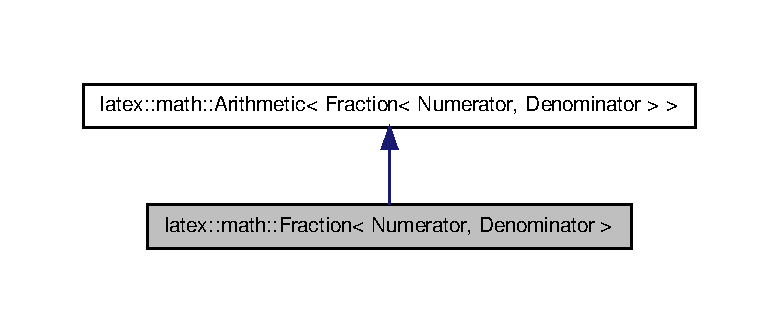
\includegraphics[width=198pt]{classlatex_1_1math_1_1Fraction__inherit__graph}
\end{center}
\end{figure}


Collaboration diagram for latex\-:\-:math\-:\-:Fraction$<$ L\-H\-S, R\-H\-S $>$\-:
\nopagebreak
\begin{figure}[H]
\begin{center}
\leavevmode
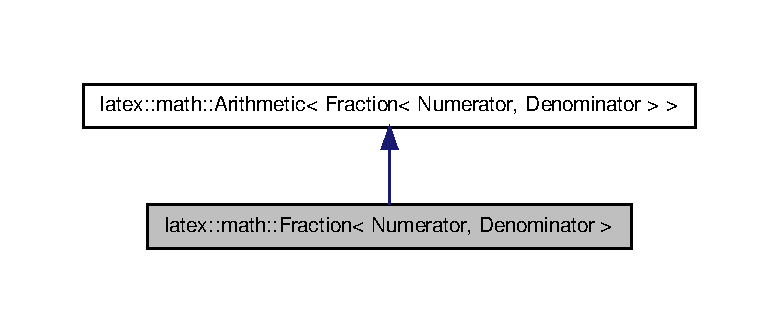
\includegraphics[width=198pt]{classlatex_1_1math_1_1Fraction__coll__graph}
\end{center}
\end{figure}
\subsection*{Public Types}
\begin{DoxyCompactItemize}
\item 
\hypertarget{classlatex_1_1math_1_1Fraction_a29f3b8b3550a01e920b5b25f7bc7993a}{using {\bfseries Numerator\-Type} = Numerator}\label{classlatex_1_1math_1_1Fraction_a29f3b8b3550a01e920b5b25f7bc7993a}

\item 
\hypertarget{classlatex_1_1math_1_1Fraction_a208b5f046738fd74662cd57e64092296}{using {\bfseries Denominator\-Type} = Denominator}\label{classlatex_1_1math_1_1Fraction_a208b5f046738fd74662cd57e64092296}

\item 
\hypertarget{classlatex_1_1math_1_1Fraction_a8b39e1eae942078b381addb7b5025d7b}{using {\bfseries Self} = \hyperlink{classlatex_1_1math_1_1Fraction}{Fraction}$<$ Numerator, Denominator $>$}\label{classlatex_1_1math_1_1Fraction_a8b39e1eae942078b381addb7b5025d7b}

\end{DoxyCompactItemize}
\subsection*{Public Member Functions}
\begin{DoxyCompactItemize}
\item 
\hypertarget{classlatex_1_1math_1_1Fraction_ac7e62595c28e64ef4fc9fb622216dbc9}{{\bfseries Fraction} (Numerator num, Denominator den)}\label{classlatex_1_1math_1_1Fraction_ac7e62595c28e64ef4fc9fb622216dbc9}

\item 
\hypertarget{classlatex_1_1math_1_1Fraction_af7a4255e44caaf99035d77d4fd66b622}{auto {\bfseries solve} ()}\label{classlatex_1_1math_1_1Fraction_af7a4255e44caaf99035d77d4fd66b622}

\item 
\hypertarget{classlatex_1_1math_1_1Fraction_a5675fc996d2830ad3bf1cee4f1d1a697}{std\-::string {\bfseries latex} () const }\label{classlatex_1_1math_1_1Fraction_a5675fc996d2830ad3bf1cee4f1d1a697}

\item 
\hypertarget{classlatex_1_1math_1_1Fraction_a994da17277ce8a0ba77036c090e28444}{{\footnotesize template$<$typename T $>$ }\\\hyperlink{classlatex_1_1math_1_1Exponent}{Exponent}$<$ \hyperlink{classlatex_1_1math_1_1Fraction}{Self}, T $>$ {\bfseries pow} (const T \&power)}\label{classlatex_1_1math_1_1Fraction_a994da17277ce8a0ba77036c090e28444}

\item 
\hypertarget{classlatex_1_1math_1_1Fraction_a080092ade7e2ef160101bc20183cc34c}{{\footnotesize template$<$typename Base $>$ }\\\hyperlink{classlatex_1_1math_1_1Log}{Log}$<$ \hyperlink{classlatex_1_1math_1_1Fraction}{Self}, Base $>$ {\bfseries log} (Base base)}\label{classlatex_1_1math_1_1Fraction_a080092ade7e2ef160101bc20183cc34c}

\item 
\hypertarget{classlatex_1_1math_1_1Fraction_a70d16ff357336b72a85d6267c62eacd0}{\hyperlink{classlatex_1_1math_1_1NaturalLog}{Natural\-Log}$<$ \hyperlink{classlatex_1_1math_1_1Fraction}{Self} $>$ {\bfseries ln} ()}\label{classlatex_1_1math_1_1Fraction_a70d16ff357336b72a85d6267c62eacd0}

\item 
\hypertarget{classlatex_1_1math_1_1Fraction_ae34b20e7e198a4e46e6ecb72a6b0aa1b}{\hyperlink{classlatex_1_1math_1_1Root}{Root}$<$ \hyperlink{classlatex_1_1math_1_1Fraction}{Self}, int $>$ {\bfseries sqrt} ()}\label{classlatex_1_1math_1_1Fraction_ae34b20e7e198a4e46e6ecb72a6b0aa1b}

\end{DoxyCompactItemize}
\subsection*{Protected Attributes}
\begin{DoxyCompactItemize}
\item 
\hypertarget{classlatex_1_1math_1_1Fraction_aadb81c77d43201c6a063777b12f6d5ad}{Numerator {\bfseries num}}\label{classlatex_1_1math_1_1Fraction_aadb81c77d43201c6a063777b12f6d5ad}

\item 
\hypertarget{classlatex_1_1math_1_1Fraction_a73c046e3d1e82e0c1189f896cda0a3a9}{Denominator {\bfseries den}}\label{classlatex_1_1math_1_1Fraction_a73c046e3d1e82e0c1189f896cda0a3a9}

\end{DoxyCompactItemize}
\subsection*{Friends}
\begin{DoxyCompactItemize}
\item 
\hypertarget{classlatex_1_1math_1_1Fraction_a9313ed58249557fab9c0b6ab5e5f977f}{std\-::ostream \& {\bfseries operator$<$$<$} (std\-::ostream \&os, const \hyperlink{classlatex_1_1math_1_1Fraction}{Fraction} \&frac)}\label{classlatex_1_1math_1_1Fraction_a9313ed58249557fab9c0b6ab5e5f977f}

\end{DoxyCompactItemize}


The documentation for this class was generated from the following file\-:\begin{DoxyCompactItemize}
\item 
latex.\-hpp\end{DoxyCompactItemize}

\hypertarget{classlatex_1_1style_1_1Huge}{\section{latex\-:\-:style\-:\-:\-Huge \-Class \-Reference}
\label{classlatex_1_1style_1_1Huge}\index{latex\-::style\-::\-Huge@{latex\-::style\-::\-Huge}}
}
\subsection*{\-Static \-Public \-Attributes}
\begin{DoxyCompactItemize}
\item 
\hypertarget{classlatex_1_1style_1_1Huge_aa51fea893411808973c2c0699b91cb23}{constexpr static const char $\ast$ {\bfseries open} = \char`\"{}$\backslash$$\backslash$huge\{\char`\"{}}\label{classlatex_1_1style_1_1Huge_aa51fea893411808973c2c0699b91cb23}

\item 
\hypertarget{classlatex_1_1style_1_1Huge_ad9abb5e698a0e3cfaeac3534a0376dc6}{constexpr static const char $\ast$ {\bfseries close} = \char`\"{}\}\char`\"{}}\label{classlatex_1_1style_1_1Huge_ad9abb5e698a0e3cfaeac3534a0376dc6}

\end{DoxyCompactItemize}


\-The documentation for this class was generated from the following file\-:\begin{DoxyCompactItemize}
\item 
latex.\-hpp\end{DoxyCompactItemize}

\hypertarget{classlatex_1_1style_1_1Huger}{\section{latex\-:\-:style\-:\-:Huger Class Reference}
\label{classlatex_1_1style_1_1Huger}\index{latex\-::style\-::\-Huger@{latex\-::style\-::\-Huger}}
}
\subsection*{Static Public Attributes}
\begin{DoxyCompactItemize}
\item 
\hypertarget{classlatex_1_1style_1_1Huger_a87ec955bda49bd2d90115e03dc4b99d2}{constexpr static const char $\ast$ {\bfseries open} = \char`\"{}\textbackslash{}\textbackslash{}Huge\{\char`\"{}}\label{classlatex_1_1style_1_1Huger_a87ec955bda49bd2d90115e03dc4b99d2}

\item 
\hypertarget{classlatex_1_1style_1_1Huger_a24d1bf39b9473b2b30e6cb8c2929637b}{constexpr static const char $\ast$ {\bfseries close} = \char`\"{}\}\char`\"{}}\label{classlatex_1_1style_1_1Huger_a24d1bf39b9473b2b30e6cb8c2929637b}

\end{DoxyCompactItemize}


The documentation for this class was generated from the following file\-:\begin{DoxyCompactItemize}
\item 
latex.\-hpp\end{DoxyCompactItemize}

\hypertarget{classlatex_1_1style_1_1Italic}{\section{latex\-:\-:style\-:\-:Italic Class Reference}
\label{classlatex_1_1style_1_1Italic}\index{latex\-::style\-::\-Italic@{latex\-::style\-::\-Italic}}
}
\subsection*{Static Public Attributes}
\begin{DoxyCompactItemize}
\item 
\hypertarget{classlatex_1_1style_1_1Italic_a9dacb3fa2bda2a9efc06cbe306b8a1a2}{constexpr static const char $\ast$ {\bfseries open} = \char`\"{}\textbackslash{}\textbackslash{}textit\{\char`\"{}}\label{classlatex_1_1style_1_1Italic_a9dacb3fa2bda2a9efc06cbe306b8a1a2}

\item 
\hypertarget{classlatex_1_1style_1_1Italic_af84fcee42a6e6a9b49de0cba5276e609}{constexpr static const char $\ast$ {\bfseries close} = \char`\"{}\}\char`\"{}}\label{classlatex_1_1style_1_1Italic_af84fcee42a6e6a9b49de0cba5276e609}

\end{DoxyCompactItemize}


The documentation for this class was generated from the following file\-:\begin{DoxyCompactItemize}
\item 
latex.\-hpp\end{DoxyCompactItemize}

\hypertarget{classlatex_1_1math_1_1style_1_1Italic}{\section{latex\-:\-:math\-:\-:style\-:\-:Italic Class Reference}
\label{classlatex_1_1math_1_1style_1_1Italic}\index{latex\-::math\-::style\-::\-Italic@{latex\-::math\-::style\-::\-Italic}}
}
\subsection*{Static Public Attributes}
\begin{DoxyCompactItemize}
\item 
\hypertarget{classlatex_1_1math_1_1style_1_1Italic_ae4fe085f6fa089c2b02d730f29bcefdf}{constexpr static const char $\ast$ {\bfseries open} = \char`\"{}\textbackslash{}\textbackslash{}mathit\{\char`\"{}}\label{classlatex_1_1math_1_1style_1_1Italic_ae4fe085f6fa089c2b02d730f29bcefdf}

\item 
\hypertarget{classlatex_1_1math_1_1style_1_1Italic_af0231e0f1e907b38e9e1db90c67686dd}{constexpr static const char $\ast$ {\bfseries close} = \char`\"{}\}\char`\"{}}\label{classlatex_1_1math_1_1style_1_1Italic_af0231e0f1e907b38e9e1db90c67686dd}

\end{DoxyCompactItemize}


The documentation for this class was generated from the following file\-:\begin{DoxyCompactItemize}
\item 
latex.\-hpp\end{DoxyCompactItemize}

\hypertarget{classlatex_1_1style_1_1Large}{\section{latex\-:\-:style\-:\-:\-Large \-Class \-Reference}
\label{classlatex_1_1style_1_1Large}\index{latex\-::style\-::\-Large@{latex\-::style\-::\-Large}}
}
\subsection*{\-Static \-Public \-Attributes}
\begin{DoxyCompactItemize}
\item 
\hypertarget{classlatex_1_1style_1_1Large_aeda83a01ded8b49a2952336684c01ce8}{constexpr static const char $\ast$ {\bfseries open} = \char`\"{}$\backslash$$\backslash$large\{\char`\"{}}\label{classlatex_1_1style_1_1Large_aeda83a01ded8b49a2952336684c01ce8}

\item 
\hypertarget{classlatex_1_1style_1_1Large_a7920d55c91d0975f916bb07d49e3d8e8}{constexpr static const char $\ast$ {\bfseries close} = \char`\"{}\}\char`\"{}}\label{classlatex_1_1style_1_1Large_a7920d55c91d0975f916bb07d49e3d8e8}

\end{DoxyCompactItemize}


\-The documentation for this class was generated from the following file\-:\begin{DoxyCompactItemize}
\item 
latex.\-hpp\end{DoxyCompactItemize}

\hypertarget{classlatex_1_1style_1_1Larger}{\section{latex\-:\-:style\-:\-:\-Larger \-Class \-Reference}
\label{classlatex_1_1style_1_1Larger}\index{latex\-::style\-::\-Larger@{latex\-::style\-::\-Larger}}
}
\subsection*{\-Static \-Public \-Attributes}
\begin{DoxyCompactItemize}
\item 
\hypertarget{classlatex_1_1style_1_1Larger_aa4c8be118e5c74db90d8040a2a8c9c89}{constexpr static const char $\ast$ {\bfseries open} = \char`\"{}$\backslash$$\backslash$\-Large\{\char`\"{}}\label{classlatex_1_1style_1_1Larger_aa4c8be118e5c74db90d8040a2a8c9c89}

\item 
\hypertarget{classlatex_1_1style_1_1Larger_aa49797027b270c812f5c7ac409567e72}{constexpr static const char $\ast$ {\bfseries close} = \char`\"{}\}\char`\"{}}\label{classlatex_1_1style_1_1Larger_aa49797027b270c812f5c7ac409567e72}

\end{DoxyCompactItemize}


\-The documentation for this class was generated from the following file\-:\begin{DoxyCompactItemize}
\item 
latex.\-hpp\end{DoxyCompactItemize}

\hypertarget{classlatex_1_1style_1_1Largest}{\section{latex\-:\-:style\-:\-:\-Largest \-Class \-Reference}
\label{classlatex_1_1style_1_1Largest}\index{latex\-::style\-::\-Largest@{latex\-::style\-::\-Largest}}
}
\subsection*{\-Static \-Public \-Attributes}
\begin{DoxyCompactItemize}
\item 
\hypertarget{classlatex_1_1style_1_1Largest_adbb0b19eadf9f950f410b654d6f8ba05}{constexpr static const char $\ast$ {\bfseries open} = \char`\"{}$\backslash$$\backslash$\-L\-A\-R\-G\-E\{\char`\"{}}\label{classlatex_1_1style_1_1Largest_adbb0b19eadf9f950f410b654d6f8ba05}

\item 
\hypertarget{classlatex_1_1style_1_1Largest_a678cae6a7d34ed7d6e7f87bd966a81fd}{constexpr static const char $\ast$ {\bfseries close} = \char`\"{}\}\char`\"{}}\label{classlatex_1_1style_1_1Largest_a678cae6a7d34ed7d6e7f87bd966a81fd}

\end{DoxyCompactItemize}


\-The documentation for this class was generated from the following file\-:\begin{DoxyCompactItemize}
\item 
latex.\-hpp\end{DoxyCompactItemize}

\hypertarget{classlatex_1_1doc_1_1List}{\section{latex\-:\-:doc\-:\-:\-List$<$ \-Style $>$ \-Class \-Template \-Reference}
\label{classlatex_1_1doc_1_1List}\index{latex\-::doc\-::\-List$<$ Style $>$@{latex\-::doc\-::\-List$<$ Style $>$}}
}


{\ttfamily \#include $<$latex.\-hpp$>$}

\subsection*{\-Public \-Member \-Functions}
\begin{DoxyCompactItemize}
\item 
\hypertarget{classlatex_1_1doc_1_1List_afd9fcb1586fd4103801d68345dc3d961}{\hyperlink{classlatex_1_1doc_1_1List}{\-List}$<$ \-Style $>$ \& {\bfseries operator$<$$<$} (const char $\ast$val)}\label{classlatex_1_1doc_1_1List_afd9fcb1586fd4103801d68345dc3d961}

\item 
\hypertarget{classlatex_1_1doc_1_1List_a403fcb27a8d89d845ca609caf2d130ac}{\hyperlink{classlatex_1_1doc_1_1List}{\-List}$<$ \-Style $>$ \& {\bfseries operator$<$$<$} (const std\-::string \&val)}\label{classlatex_1_1doc_1_1List_a403fcb27a8d89d845ca609caf2d130ac}

\item 
\hypertarget{classlatex_1_1doc_1_1List_ad269a03ad06439356e17c86582b03297}{\hyperlink{classlatex_1_1doc_1_1List}{\-List}$<$ \-Style $>$ \& {\bfseries operator$<$$<$} (\hyperlink{classlatex_1_1doc_1_1List}{\-List}$<$ \-Style $>$ \&val)}\label{classlatex_1_1doc_1_1List_ad269a03ad06439356e17c86582b03297}

\item 
\hypertarget{classlatex_1_1doc_1_1List_af2f4cbc14d4001b7e185392d8cddf9e8}{\hyperlink{classlatex_1_1doc_1_1List}{\-List}$<$ \-Style $>$ \& {\bfseries operator$<$$<$} (const \hyperlink{classlatex_1_1doc_1_1List}{\-List}$<$ \-Style $>$ \&val)}\label{classlatex_1_1doc_1_1List_af2f4cbc14d4001b7e185392d8cddf9e8}

\item 
\hypertarget{classlatex_1_1doc_1_1List_a9a5ed93557cd28c325cec55fcf74c76c}{{\footnotesize template$<$typename T , typename  = typename std\-::enable\-\_\-if$<$                can\-\_\-stringify$<$\-T$>$\-::value                and                (not std\-::is\-\_\-same$<$\-T, List$<$listtypes\-::\-Ordered$>$$>$\-::value and not std\-::is\-\_\-same$<$\-T, List$<$listtypes\-::\-Unordered$>$$>$\-::value)            $>$\-::type$>$ }\\\hyperlink{classlatex_1_1doc_1_1List}{\-List}$<$ \-Style $>$ \& {\bfseries operator$<$$<$} (const \-T \&val)}\label{classlatex_1_1doc_1_1List_a9a5ed93557cd28c325cec55fcf74c76c}

\item 
\hypertarget{classlatex_1_1doc_1_1List_a68d596e7d17e04cfabbc06d80a954940}{{\footnotesize template$<$typename T $>$ }\\std\-::enable\-\_\-if$<$ can\-\_\-latex$<$ \-T $>$\*
\-::value, \hyperlink{classlatex_1_1doc_1_1List}{\-List}$<$ \-Style $>$\*
 \& $>$\-::type {\bfseries operator$<$$<$} (const \-T \&val)}\label{classlatex_1_1doc_1_1List_a68d596e7d17e04cfabbc06d80a954940}

\item 
\hypertarget{classlatex_1_1doc_1_1List_a04b52890de459bc6c6d0a6741b55bdf7}{void {\bfseries add} (const std\-::string \&str)}\label{classlatex_1_1doc_1_1List_a04b52890de459bc6c6d0a6741b55bdf7}

\item 
\hypertarget{classlatex_1_1doc_1_1List_a720d7827235c61d025ff66ed4723b0e9}{void {\bfseries add\-\_\-sublist} (const \hyperlink{classlatex_1_1doc_1_1List}{\-List}$<$ \-Style $>$ \&list)}\label{classlatex_1_1doc_1_1List_a720d7827235c61d025ff66ed4723b0e9}

\item 
\hypertarget{classlatex_1_1doc_1_1List_a5000125c08e3837c03f766f30a429cb1}{std\-::string {\bfseries to\-\_\-string} () const }\label{classlatex_1_1doc_1_1List_a5000125c08e3837c03f766f30a429cb1}

\item 
\hypertarget{classlatex_1_1doc_1_1List_a5ea2a813625fbeb5752ea66a12ac0a59}{void {\bfseries build} (std\-::ostream \&os, std\-::size\-\_\-t depth=1) const }\label{classlatex_1_1doc_1_1List_a5ea2a813625fbeb5752ea66a12ac0a59}

\end{DoxyCompactItemize}
\subsection*{\-Public \-Attributes}
\begin{DoxyCompactItemize}
\item 
\hypertarget{classlatex_1_1doc_1_1List_adacc628c072f9be831cab48615b8b564}{std\-::vector$<$ std\-::string $>$ {\bfseries items}}\label{classlatex_1_1doc_1_1List_adacc628c072f9be831cab48615b8b564}

\item 
\hypertarget{classlatex_1_1doc_1_1List_ac1ee0ddbd69ab8dfc46ae6f5fbdc21a1}{std\-::vector$<$ \hyperlink{classlatex_1_1doc_1_1List}{\-List}$<$ \-Style $>$ $>$ {\bfseries sublists}}\label{classlatex_1_1doc_1_1List_ac1ee0ddbd69ab8dfc46ae6f5fbdc21a1}

\end{DoxyCompactItemize}
\subsection*{\-Protected \-Types}
\begin{DoxyCompactItemize}
\item 
enum {\bfseries \-Entry\-Type} \{ {\bfseries \-String}, 
{\bfseries \-Sublist}
 \}
\end{DoxyCompactItemize}
\subsection*{\-Protected \-Attributes}
\begin{DoxyCompactItemize}
\item 
\hypertarget{classlatex_1_1doc_1_1List_ae8e20e36cd4a198bd9062d5fe7578f00}{std\-::vector$<$ \-Entry\-Type $>$ {\bfseries ordering}}\label{classlatex_1_1doc_1_1List_ae8e20e36cd4a198bd9062d5fe7578f00}

\end{DoxyCompactItemize}
\subsection*{\-Friends}
\begin{DoxyCompactItemize}
\item 
\hypertarget{classlatex_1_1doc_1_1List_a9cf2b64b3af2172b2feedf0b75bda63d}{std\-::ostream \& {\bfseries operator$<$$<$} (std\-::ostream \&os, \hyperlink{classlatex_1_1doc_1_1List}{\-List} \&list)}\label{classlatex_1_1doc_1_1List_a9cf2b64b3af2172b2feedf0b75bda63d}

\end{DoxyCompactItemize}


\subsection{\-Detailed \-Description}
\subsubsection*{template$<$typename \-Style = listtypes\-::\-Unordered$>$class latex\-::doc\-::\-List$<$ Style $>$}

\-Create a \-La\-Te\-X formatted list.

\-Nested lists must be of the same style (i.\-e. cannot mix \-Ordered and \-Unordered). 

\-The documentation for this class was generated from the following file\-:\begin{DoxyCompactItemize}
\item 
latex.\-hpp\end{DoxyCompactItemize}

\hypertarget{classlatex_1_1math_1_1Log}{\section{latex\-:\-:math\-:\-:\-Log$<$ \-Val, \-Base $>$ \-Class \-Template \-Reference}
\label{classlatex_1_1math_1_1Log}\index{latex\-::math\-::\-Log$<$ Val, Base $>$@{latex\-::math\-::\-Log$<$ Val, Base $>$}}
}


\-Inheritance diagram for latex\-:\-:math\-:\-:\-Log$<$ \-Val, \-Base $>$\-:
\nopagebreak
\begin{figure}[H]
\begin{center}
\leavevmode
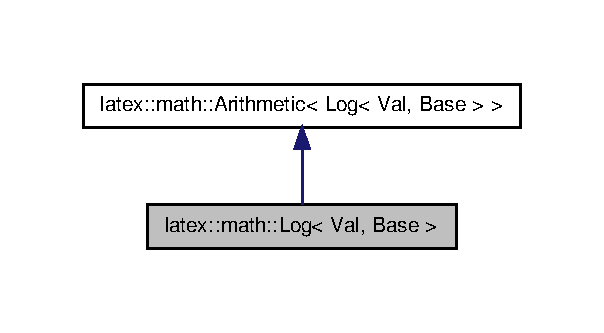
\includegraphics[width=290pt]{classlatex_1_1math_1_1Log__inherit__graph}
\end{center}
\end{figure}


\-Collaboration diagram for latex\-:\-:math\-:\-:\-Log$<$ \-Val, \-Base $>$\-:
\nopagebreak
\begin{figure}[H]
\begin{center}
\leavevmode
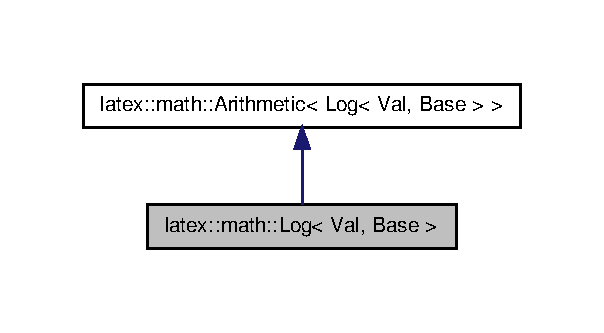
\includegraphics[width=290pt]{classlatex_1_1math_1_1Log__coll__graph}
\end{center}
\end{figure}
\subsection*{\-Public \-Member \-Functions}
\begin{DoxyCompactItemize}
\item 
\hypertarget{classlatex_1_1math_1_1Log_acff6d6f36adff38cf7c0da719516c6bc}{{\bfseries \-Log} (\-Val val, \-Base base)}\label{classlatex_1_1math_1_1Log_acff6d6f36adff38cf7c0da719516c6bc}

\item 
\hypertarget{classlatex_1_1math_1_1Log_a5d9819331208c23d8978a3744d058f14}{auto {\bfseries solve} ()}\label{classlatex_1_1math_1_1Log_a5d9819331208c23d8978a3744d058f14}

\item 
\hypertarget{classlatex_1_1math_1_1Log_a1bc90c91e52e7858e33dcdaba673b7a9}{std\-::string {\bfseries latex} () const }\label{classlatex_1_1math_1_1Log_a1bc90c91e52e7858e33dcdaba673b7a9}

\item 
\hypertarget{classlatex_1_1math_1_1Log_a4819a4a9a01dd7dd65a0d2773c589976}{{\footnotesize template$<$typename T $>$ }\\\hyperlink{classlatex_1_1math_1_1Exponent}{\-Exponent}$<$ \-Self, \-T $>$ {\bfseries pow} (const \-T \&power)}\label{classlatex_1_1math_1_1Log_a4819a4a9a01dd7dd65a0d2773c589976}

\item 
\hypertarget{classlatex_1_1math_1_1Log_aacf7a5312839b22b33fcb67ed3f51fde}{{\footnotesize template$<$typename Inner\-Base $>$ }\\\hyperlink{classlatex_1_1math_1_1Log}{\-Log}$<$ \-Self, \-Base $>$ {\bfseries log} ()}\label{classlatex_1_1math_1_1Log_aacf7a5312839b22b33fcb67ed3f51fde}

\item 
\hypertarget{classlatex_1_1math_1_1Log_a6ae7bf3b1ce862280b67b58f69d5c793}{\hyperlink{classlatex_1_1math_1_1NaturalLog}{\-Natural\-Log}$<$ \-Self $>$ {\bfseries ln} ()}\label{classlatex_1_1math_1_1Log_a6ae7bf3b1ce862280b67b58f69d5c793}

\item 
\hypertarget{classlatex_1_1math_1_1Log_a980f02ee52b6b81f1c7e7ccf75521a67}{\hyperlink{classlatex_1_1math_1_1Root}{\-Root}$<$ \-Self, int $>$ {\bfseries sqrt} ()}\label{classlatex_1_1math_1_1Log_a980f02ee52b6b81f1c7e7ccf75521a67}

\end{DoxyCompactItemize}
\subsection*{\-Protected \-Attributes}
\begin{DoxyCompactItemize}
\item 
\hypertarget{classlatex_1_1math_1_1Log_a7f4ac09a355183bcec59b0f7fe686f43}{\-Val {\bfseries val}}\label{classlatex_1_1math_1_1Log_a7f4ac09a355183bcec59b0f7fe686f43}

\item 
\hypertarget{classlatex_1_1math_1_1Log_a487bc150b50dd56998b2541ae5c335ab}{\-Base {\bfseries base}}\label{classlatex_1_1math_1_1Log_a487bc150b50dd56998b2541ae5c335ab}

\end{DoxyCompactItemize}
\subsection*{\-Friends}
\begin{DoxyCompactItemize}
\item 
\hypertarget{classlatex_1_1math_1_1Log_ab9f88137b0d5fb0ab0f04bf4003514fe}{std\-::ostream \& {\bfseries operator$<$$<$} (std\-::ostream \&os, const \hyperlink{classlatex_1_1math_1_1Log}{\-Log} \&loga)}\label{classlatex_1_1math_1_1Log_ab9f88137b0d5fb0ab0f04bf4003514fe}

\end{DoxyCompactItemize}
\subsubsection*{template$<$typename \-Val, typename \-Base = \-Val$>$ class latex\-::math\-::\-Log$<$ Val, Base $>$}



\-The documentation for this class was generated from the following file\-:\begin{DoxyCompactItemize}
\item 
latex.\-hpp\end{DoxyCompactItemize}

\hypertarget{classlatex_1_1math_1_1Multiplication}{\section{latex\-:\-:math\-:\-:Multiplication$<$ L\-H\-S, R\-H\-S $>$ Class Template Reference}
\label{classlatex_1_1math_1_1Multiplication}\index{latex\-::math\-::\-Multiplication$<$ L\-H\-S, R\-H\-S $>$@{latex\-::math\-::\-Multiplication$<$ L\-H\-S, R\-H\-S $>$}}
}
\subsection*{Public Types}
\begin{DoxyCompactItemize}
\item 
\hypertarget{classlatex_1_1math_1_1Multiplication_a78215162923b7966cae1e4a360560668}{using {\bfseries L\-H\-S\-Type} = L\-H\-S}\label{classlatex_1_1math_1_1Multiplication_a78215162923b7966cae1e4a360560668}

\item 
\hypertarget{classlatex_1_1math_1_1Multiplication_ad505c00cdcc46719478e3199854f2b0b}{using {\bfseries R\-H\-S\-Type} = R\-H\-S}\label{classlatex_1_1math_1_1Multiplication_ad505c00cdcc46719478e3199854f2b0b}

\item 
\hypertarget{classlatex_1_1math_1_1Multiplication_a6e50f629d0cd2719816ca3b6b80fefd0}{using {\bfseries Self} = \hyperlink{classlatex_1_1math_1_1Multiplication}{Multiplication}$<$ L\-H\-S, R\-H\-S $>$}\label{classlatex_1_1math_1_1Multiplication_a6e50f629d0cd2719816ca3b6b80fefd0}

\end{DoxyCompactItemize}
\subsection*{Public Member Functions}
\begin{DoxyCompactItemize}
\item 
\hypertarget{classlatex_1_1math_1_1Multiplication_a01b926587f44a050634d8f79d7ff7714}{{\bfseries Multiplication} (L\-H\-S lhs, R\-H\-S rhs)}\label{classlatex_1_1math_1_1Multiplication_a01b926587f44a050634d8f79d7ff7714}

\item 
\hypertarget{classlatex_1_1math_1_1Multiplication_a29577e0e2321b539428a023ac60e360c}{auto {\bfseries solve} ()}\label{classlatex_1_1math_1_1Multiplication_a29577e0e2321b539428a023ac60e360c}

\item 
\hypertarget{classlatex_1_1math_1_1Multiplication_a658d8f7990c84934f66de6b604349f02}{std\-::string {\bfseries latex} () const }\label{classlatex_1_1math_1_1Multiplication_a658d8f7990c84934f66de6b604349f02}

\item 
\hypertarget{classlatex_1_1math_1_1Multiplication_a522397a5a3c8f67e67cf8e72b9818550}{{\footnotesize template$<$typename T $>$ }\\\hyperlink{classlatex_1_1math_1_1Power}{Power}$<$ \hyperlink{classlatex_1_1math_1_1Multiplication}{Self}, T $>$ {\bfseries pow} (const T \&power)}\label{classlatex_1_1math_1_1Multiplication_a522397a5a3c8f67e67cf8e72b9818550}

\item 
\hypertarget{classlatex_1_1math_1_1Multiplication_ae0ad97bbdf076e41566b2383d748edfb}{{\footnotesize template$<$typename Base $>$ }\\\hyperlink{classlatex_1_1math_1_1Log}{Log}$<$ \hyperlink{classlatex_1_1math_1_1Multiplication}{Self}, Base $>$ {\bfseries log} (Base base)}\label{classlatex_1_1math_1_1Multiplication_ae0ad97bbdf076e41566b2383d748edfb}

\item 
\hypertarget{classlatex_1_1math_1_1Multiplication_a33c4db51176ef8a04234a5ec27c05387}{\hyperlink{classlatex_1_1math_1_1NaturalLog}{Natural\-Log}$<$ \hyperlink{classlatex_1_1math_1_1Multiplication}{Self} $>$ {\bfseries ln} ()}\label{classlatex_1_1math_1_1Multiplication_a33c4db51176ef8a04234a5ec27c05387}

\item 
\hypertarget{classlatex_1_1math_1_1Multiplication_af67f7c4a1d4898681a87826a53b98099}{\hyperlink{classlatex_1_1math_1_1Root}{Root}$<$ \hyperlink{classlatex_1_1math_1_1Multiplication}{Self}, int $>$ {\bfseries sqrt} ()}\label{classlatex_1_1math_1_1Multiplication_af67f7c4a1d4898681a87826a53b98099}

\end{DoxyCompactItemize}
\subsection*{Protected Attributes}
\begin{DoxyCompactItemize}
\item 
\hypertarget{classlatex_1_1math_1_1Multiplication_a4023853877f13a570cb9b576f92fa5ee}{L\-H\-S {\bfseries lhs}}\label{classlatex_1_1math_1_1Multiplication_a4023853877f13a570cb9b576f92fa5ee}

\item 
\hypertarget{classlatex_1_1math_1_1Multiplication_a032c65778b9166b745136e6b6349a064}{R\-H\-S {\bfseries rhs}}\label{classlatex_1_1math_1_1Multiplication_a032c65778b9166b745136e6b6349a064}

\end{DoxyCompactItemize}
\subsection*{Friends}
\begin{DoxyCompactItemize}
\item 
\hypertarget{classlatex_1_1math_1_1Multiplication_ad1e78a956a232d4eb730bd2fef03ea65}{std\-::ostream \& {\bfseries operator$<$$<$} (std\-::ostream \&os, const \hyperlink{classlatex_1_1math_1_1Multiplication}{Multiplication} \&mult)}\label{classlatex_1_1math_1_1Multiplication_ad1e78a956a232d4eb730bd2fef03ea65}

\end{DoxyCompactItemize}


The documentation for this class was generated from the following file\-:\begin{DoxyCompactItemize}
\item 
latex.\-hpp\end{DoxyCompactItemize}

\hypertarget{classlatex_1_1math_1_1NaturalLog}{\section{latex\-:\-:math\-:\-:Natural\-Log$<$ Val $>$ Class Template Reference}
\label{classlatex_1_1math_1_1NaturalLog}\index{latex\-::math\-::\-Natural\-Log$<$ Val $>$@{latex\-::math\-::\-Natural\-Log$<$ Val $>$}}
}


Inheritance diagram for latex\-:\-:math\-:\-:Natural\-Log$<$ Val $>$\-:
\nopagebreak
\begin{figure}[H]
\begin{center}
\leavevmode
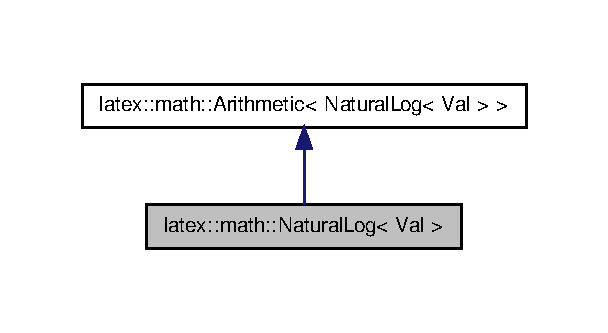
\includegraphics[width=198pt]{classlatex_1_1math_1_1NaturalLog__inherit__graph}
\end{center}
\end{figure}


Collaboration diagram for latex\-:\-:math\-:\-:Natural\-Log$<$ Val $>$\-:
\nopagebreak
\begin{figure}[H]
\begin{center}
\leavevmode
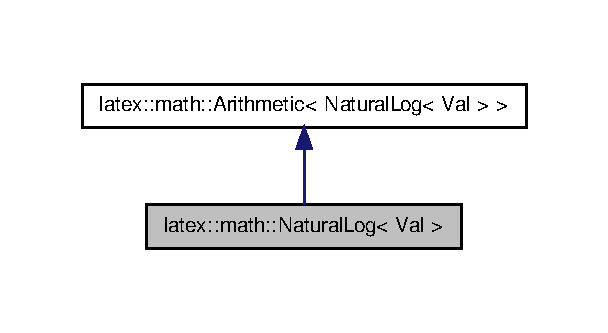
\includegraphics[width=198pt]{classlatex_1_1math_1_1NaturalLog__coll__graph}
\end{center}
\end{figure}
\subsection*{Public Types}
\begin{DoxyCompactItemize}
\item 
\hypertarget{classlatex_1_1math_1_1NaturalLog_a3c4e70fee11fb15ab7b15957fdad497d}{using {\bfseries Val\-Type} = Val}\label{classlatex_1_1math_1_1NaturalLog_a3c4e70fee11fb15ab7b15957fdad497d}

\item 
\hypertarget{classlatex_1_1math_1_1NaturalLog_a7a95f61ac1bac6dba31c940aeb81ba34}{using {\bfseries Self} = \hyperlink{classlatex_1_1math_1_1NaturalLog}{Natural\-Log}$<$ Val $>$}\label{classlatex_1_1math_1_1NaturalLog_a7a95f61ac1bac6dba31c940aeb81ba34}

\end{DoxyCompactItemize}
\subsection*{Public Member Functions}
\begin{DoxyCompactItemize}
\item 
\hypertarget{classlatex_1_1math_1_1NaturalLog_aeeb12e56e32d76ced7fbd41e82941d0f}{{\bfseries Natural\-Log} (Val val)}\label{classlatex_1_1math_1_1NaturalLog_aeeb12e56e32d76ced7fbd41e82941d0f}

\item 
\hypertarget{classlatex_1_1math_1_1NaturalLog_ad4ffac52939e962b891122008b323abf}{auto {\bfseries solve} ()}\label{classlatex_1_1math_1_1NaturalLog_ad4ffac52939e962b891122008b323abf}

\item 
\hypertarget{classlatex_1_1math_1_1NaturalLog_af75e70ab4e10082741e89127ead0a32b}{std\-::string {\bfseries latex} () const }\label{classlatex_1_1math_1_1NaturalLog_af75e70ab4e10082741e89127ead0a32b}

\item 
\hypertarget{classlatex_1_1math_1_1NaturalLog_a94d5f44f2bb1000ae0a969cccc781bb4}{{\footnotesize template$<$typename T $>$ }\\\hyperlink{classlatex_1_1math_1_1Exponent}{Exponent}$<$ \hyperlink{classlatex_1_1math_1_1NaturalLog}{Self}, T $>$ {\bfseries pow} (const T \&power)}\label{classlatex_1_1math_1_1NaturalLog_a94d5f44f2bb1000ae0a969cccc781bb4}

\item 
\hypertarget{classlatex_1_1math_1_1NaturalLog_abea6ea1be29c3e5bbbabbcf758a79fbf}{{\footnotesize template$<$typename Base $>$ }\\\hyperlink{classlatex_1_1math_1_1Log}{Log}$<$ \hyperlink{classlatex_1_1math_1_1NaturalLog}{Self}, Base $>$ {\bfseries log} (Base base)}\label{classlatex_1_1math_1_1NaturalLog_abea6ea1be29c3e5bbbabbcf758a79fbf}

\item 
\hypertarget{classlatex_1_1math_1_1NaturalLog_ae8720764dd2a28eae1133eb7d5e584b8}{\hyperlink{classlatex_1_1math_1_1NaturalLog}{Natural\-Log}$<$ \hyperlink{classlatex_1_1math_1_1NaturalLog}{Self} $>$ {\bfseries ln} ()}\label{classlatex_1_1math_1_1NaturalLog_ae8720764dd2a28eae1133eb7d5e584b8}

\item 
\hypertarget{classlatex_1_1math_1_1NaturalLog_aa73f79ce7b2acb561a8bc190d585c7a8}{\hyperlink{classlatex_1_1math_1_1Root}{Root}$<$ \hyperlink{classlatex_1_1math_1_1NaturalLog}{Self}, int $>$ {\bfseries sqrt} ()}\label{classlatex_1_1math_1_1NaturalLog_aa73f79ce7b2acb561a8bc190d585c7a8}

\end{DoxyCompactItemize}
\subsection*{Protected Attributes}
\begin{DoxyCompactItemize}
\item 
\hypertarget{classlatex_1_1math_1_1NaturalLog_a46cee76970936d26daf87e8c3ec4c47b}{Val {\bfseries val}}\label{classlatex_1_1math_1_1NaturalLog_a46cee76970936d26daf87e8c3ec4c47b}

\end{DoxyCompactItemize}
\subsection*{Friends}
\begin{DoxyCompactItemize}
\item 
\hypertarget{classlatex_1_1math_1_1NaturalLog_a5151466531baf2bea2fc1928e34cb084}{std\-::ostream \& {\bfseries operator$<$$<$} (std\-::ostream \&os, const \hyperlink{classlatex_1_1math_1_1NaturalLog}{Natural\-Log} \&loga)}\label{classlatex_1_1math_1_1NaturalLog_a5151466531baf2bea2fc1928e34cb084}

\end{DoxyCompactItemize}


The documentation for this class was generated from the following file\-:\begin{DoxyCompactItemize}
\item 
latex.\-hpp\end{DoxyCompactItemize}

\hypertarget{classlatex_1_1math_1_1style_1_1None}{\section{latex\-:\-:math\-:\-:style\-:\-:None Class Reference}
\label{classlatex_1_1math_1_1style_1_1None}\index{latex\-::math\-::style\-::\-None@{latex\-::math\-::style\-::\-None}}
}
\subsection*{Static Public Attributes}
\begin{DoxyCompactItemize}
\item 
\hypertarget{classlatex_1_1math_1_1style_1_1None_ab89a30cf0012d035336c200f458db817}{constexpr static const char $\ast$ {\bfseries open} = \char`\"{}\char`\"{}}\label{classlatex_1_1math_1_1style_1_1None_ab89a30cf0012d035336c200f458db817}

\item 
\hypertarget{classlatex_1_1math_1_1style_1_1None_a0a141edba881d2fc1132969f7c418c56}{constexpr static const char $\ast$ {\bfseries close} = \char`\"{}\char`\"{}}\label{classlatex_1_1math_1_1style_1_1None_a0a141edba881d2fc1132969f7c418c56}

\end{DoxyCompactItemize}


The documentation for this class was generated from the following file\-:\begin{DoxyCompactItemize}
\item 
latex.\-hpp\end{DoxyCompactItemize}

\hypertarget{classlatex_1_1style_1_1None}{\section{latex\-:\-:style\-:\-:\-None \-Class \-Reference}
\label{classlatex_1_1style_1_1None}\index{latex\-::style\-::\-None@{latex\-::style\-::\-None}}
}
\subsection*{\-Static \-Public \-Attributes}
\begin{DoxyCompactItemize}
\item 
\hypertarget{classlatex_1_1style_1_1None_a742bf0986955725b3cbe15bbb889cec9}{constexpr static const char $\ast$ {\bfseries open} = \char`\"{}\char`\"{}}\label{classlatex_1_1style_1_1None_a742bf0986955725b3cbe15bbb889cec9}

\item 
\hypertarget{classlatex_1_1style_1_1None_aafb4d115dc87e0ae25cc5a38a49e9f38}{constexpr static const char $\ast$ {\bfseries close} = \char`\"{}\char`\"{}}\label{classlatex_1_1style_1_1None_aafb4d115dc87e0ae25cc5a38a49e9f38}

\end{DoxyCompactItemize}


\-The documentation for this class was generated from the following file\-:\begin{DoxyCompactItemize}
\item 
latex.\-hpp\end{DoxyCompactItemize}

\hypertarget{classlatex_1_1style_1_1Normal}{\section{latex\-:\-:style\-:\-:Normal Class Reference}
\label{classlatex_1_1style_1_1Normal}\index{latex\-::style\-::\-Normal@{latex\-::style\-::\-Normal}}
}
\subsection*{Static Public Attributes}
\begin{DoxyCompactItemize}
\item 
\hypertarget{classlatex_1_1style_1_1Normal_ab91741000604603ad79213748fb365d0}{constexpr static const char $\ast$ {\bfseries open} = \char`\"{}\textbackslash{}\textbackslash{}normal\{\char`\"{}}\label{classlatex_1_1style_1_1Normal_ab91741000604603ad79213748fb365d0}

\item 
\hypertarget{classlatex_1_1style_1_1Normal_abc6bcd5cfedf7007237468bad885fa6a}{constexpr static const char $\ast$ {\bfseries close} = \char`\"{}\}\char`\"{}}\label{classlatex_1_1style_1_1Normal_abc6bcd5cfedf7007237468bad885fa6a}

\end{DoxyCompactItemize}


The documentation for this class was generated from the following file\-:\begin{DoxyCompactItemize}
\item 
latex.\-hpp\end{DoxyCompactItemize}

\hypertarget{classlatex_1_1math_1_1style_1_1Normal}{\section{latex\-:\-:math\-:\-:style\-:\-:Normal Class Reference}
\label{classlatex_1_1math_1_1style_1_1Normal}\index{latex\-::math\-::style\-::\-Normal@{latex\-::math\-::style\-::\-Normal}}
}
\subsection*{Static Public Attributes}
\begin{DoxyCompactItemize}
\item 
\hypertarget{classlatex_1_1math_1_1style_1_1Normal_a49ee8c066a06a3d15d61c077f56cc9d1}{constexpr static const char $\ast$ {\bfseries open} = \char`\"{}\textbackslash{}\textbackslash{}mathnormal\{\char`\"{}}\label{classlatex_1_1math_1_1style_1_1Normal_a49ee8c066a06a3d15d61c077f56cc9d1}

\item 
\hypertarget{classlatex_1_1math_1_1style_1_1Normal_abd05edd097677152f5828ae1ee4bea4d}{constexpr static const char $\ast$ {\bfseries close} = \char`\"{}\}\char`\"{}}\label{classlatex_1_1math_1_1style_1_1Normal_abd05edd097677152f5828ae1ee4bea4d}

\end{DoxyCompactItemize}


The documentation for this class was generated from the following file\-:\begin{DoxyCompactItemize}
\item 
latex.\-hpp\end{DoxyCompactItemize}

\hypertarget{classlatex_1_1math_1_1Number}{\section{latex\-:\-:math\-:\-:Number$<$ T $>$ Class Template Reference}
\label{classlatex_1_1math_1_1Number}\index{latex\-::math\-::\-Number$<$ T $>$@{latex\-::math\-::\-Number$<$ T $>$}}
}


{\ttfamily \#include $<$latex.\-hpp$>$}

\subsection*{Public Types}
\begin{DoxyCompactItemize}
\item 
\hypertarget{classlatex_1_1math_1_1Number_a0ae5c2f5bd6ad61202cc71f06e8d45b5}{using {\bfseries Self} = \hyperlink{classlatex_1_1math_1_1Number}{Number}$<$ T $>$}\label{classlatex_1_1math_1_1Number_a0ae5c2f5bd6ad61202cc71f06e8d45b5}

\end{DoxyCompactItemize}
\subsection*{Public Member Functions}
\begin{DoxyCompactItemize}
\item 
\hypertarget{classlatex_1_1math_1_1Number_ad95c73319da794a949d07258f3cd23f3}{{\bfseries Number} (T val)}\label{classlatex_1_1math_1_1Number_ad95c73319da794a949d07258f3cd23f3}

\item 
\hypertarget{classlatex_1_1math_1_1Number_a828245764da36255de6fc5de3ff419cf}{auto {\bfseries solve} ()}\label{classlatex_1_1math_1_1Number_a828245764da36255de6fc5de3ff419cf}

\item 
\hypertarget{classlatex_1_1math_1_1Number_a4ba49b934f893e3582f755a2830cc9f5}{std\-::string {\bfseries latex} () const }\label{classlatex_1_1math_1_1Number_a4ba49b934f893e3582f755a2830cc9f5}

\item 
\hypertarget{classlatex_1_1math_1_1Number_a8ab91d58fe8e6708b72d53fb0266b9c9}{\hyperlink{classlatex_1_1math_1_1Number}{Self} {\bfseries operator-\/} ()}\label{classlatex_1_1math_1_1Number_a8ab91d58fe8e6708b72d53fb0266b9c9}

\item 
\hypertarget{classlatex_1_1math_1_1Number_aa2f067bcad6aa2afd7fb83faea74336a}{{\footnotesize template$<$typename Pow $>$ }\\\hyperlink{classlatex_1_1math_1_1Exponent}{Exponent}$<$ \hyperlink{classlatex_1_1math_1_1Number}{Self}, Pow $>$ {\bfseries pow} (const Pow \&power)}\label{classlatex_1_1math_1_1Number_aa2f067bcad6aa2afd7fb83faea74336a}

\item 
\hypertarget{classlatex_1_1math_1_1Number_af8ac2784e513ee0761c9a42972fc9744}{{\footnotesize template$<$typename Base $>$ }\\\hyperlink{classlatex_1_1math_1_1Log}{Log}$<$ \hyperlink{classlatex_1_1math_1_1Number}{Self}, Base $>$ {\bfseries log} (Base base)}\label{classlatex_1_1math_1_1Number_af8ac2784e513ee0761c9a42972fc9744}

\item 
\hypertarget{classlatex_1_1math_1_1Number_a5a808cf6ecbb48144d85cad64def6b42}{\hyperlink{classlatex_1_1math_1_1NaturalLog}{Natural\-Log}$<$ \hyperlink{classlatex_1_1math_1_1Number}{Self} $>$ {\bfseries ln} ()}\label{classlatex_1_1math_1_1Number_a5a808cf6ecbb48144d85cad64def6b42}

\item 
\hypertarget{classlatex_1_1math_1_1Number_a41e6361f370fe20ed6bf147807d8edb3}{\hyperlink{classlatex_1_1math_1_1Root}{Root}$<$ \hyperlink{classlatex_1_1math_1_1Number}{Self}, int $>$ {\bfseries sqrt} ()}\label{classlatex_1_1math_1_1Number_a41e6361f370fe20ed6bf147807d8edb3}

\end{DoxyCompactItemize}
\subsection*{Protected Attributes}
\begin{DoxyCompactItemize}
\item 
\hypertarget{classlatex_1_1math_1_1Number_a7a761cdf214f2d5752808ddaf651d2b7}{T {\bfseries val}}\label{classlatex_1_1math_1_1Number_a7a761cdf214f2d5752808ddaf651d2b7}

\end{DoxyCompactItemize}
\subsection*{Friends}
\begin{DoxyCompactItemize}
\item 
\hypertarget{classlatex_1_1math_1_1Number_aa6d72faef992d5b025e38cfbaad05ee4}{std\-::ostream \& {\bfseries operator$<$$<$} (std\-::ostream \&os, const \hyperlink{classlatex_1_1math_1_1Number}{Number} \&num)}\label{classlatex_1_1math_1_1Number_aa6d72faef992d5b025e38cfbaad05ee4}

\end{DoxyCompactItemize}


\subsection{Detailed Description}
\subsubsection*{template$<$typename T$>$class latex\-::math\-::\-Number$<$ T $>$}

Helper class for \char`\"{}entering the La\-Te\-X context\char`\"{} using a constant numeric.

Most commonly used to then access the overloaded operators. 

The documentation for this class was generated from the following file\-:\begin{DoxyCompactItemize}
\item 
latex.\-hpp\end{DoxyCompactItemize}

\hypertarget{classlatex_1_1doc_1_1listtypes_1_1Ordered}{\section{latex\-:\-:doc\-:\-:listtypes\-:\-:\-Ordered \-Class \-Reference}
\label{classlatex_1_1doc_1_1listtypes_1_1Ordered}\index{latex\-::doc\-::listtypes\-::\-Ordered@{latex\-::doc\-::listtypes\-::\-Ordered}}
}


{\ttfamily \#include $<$latex.\-hpp$>$}

\subsection*{\-Static \-Public \-Attributes}
\begin{DoxyCompactItemize}
\item 
\hypertarget{classlatex_1_1doc_1_1listtypes_1_1Ordered_abe82c02d83ba66d14e5b0f0301aefd36}{constexpr static const char $\ast$ {\bfseries open} = \char`\"{}$\backslash$$\backslash$begin\{enumerate\}\char`\"{}}\label{classlatex_1_1doc_1_1listtypes_1_1Ordered_abe82c02d83ba66d14e5b0f0301aefd36}

\item 
\hypertarget{classlatex_1_1doc_1_1listtypes_1_1Ordered_af9bb481a3ac6257629c086fee6124384}{constexpr static const char $\ast$ {\bfseries close} = \char`\"{}$\backslash$$\backslash$end\{enumerate\}\char`\"{}}\label{classlatex_1_1doc_1_1listtypes_1_1Ordered_af9bb481a3ac6257629c086fee6124384}

\end{DoxyCompactItemize}


\subsection{\-Detailed \-Description}
\-Specifies the list should be represented in an ordered (numbered rather than bulleted) form. 

\-The documentation for this class was generated from the following file\-:\begin{DoxyCompactItemize}
\item 
latex.\-hpp\end{DoxyCompactItemize}

\hypertarget{classlatex_1_1math_1_1Paren}{\section{latex\-:\-:math\-:\-:\-Paren$<$ \-T $>$ \-Class \-Template \-Reference}
\label{classlatex_1_1math_1_1Paren}\index{latex\-::math\-::\-Paren$<$ T $>$@{latex\-::math\-::\-Paren$<$ T $>$}}
}


{\ttfamily \#include $<$latex.\-hpp$>$}



\-Collaboration diagram for latex\-:\-:math\-:\-:\-Paren$<$ \-T $>$\-:
\subsection*{\-Public \-Member \-Functions}
\begin{DoxyCompactItemize}
\item 
\hypertarget{classlatex_1_1math_1_1Paren_a92ee4e0a519162e5c81ee889fdffb6ac}{{\bfseries \-Paren} (\-T enc)}\label{classlatex_1_1math_1_1Paren_a92ee4e0a519162e5c81ee889fdffb6ac}

\item 
\hypertarget{classlatex_1_1math_1_1Paren_aa64116c67d309121e19040fb3677da6a}{auto {\bfseries solve} ()}\label{classlatex_1_1math_1_1Paren_aa64116c67d309121e19040fb3677da6a}

\item 
\hypertarget{classlatex_1_1math_1_1Paren_a1f98ca0b80126f3df1ac5343788790ca}{std\-::string {\bfseries latex} () const }\label{classlatex_1_1math_1_1Paren_a1f98ca0b80126f3df1ac5343788790ca}

\end{DoxyCompactItemize}
\subsection*{\-Public \-Attributes}
\begin{DoxyCompactItemize}
\item 
\hypertarget{classlatex_1_1math_1_1Paren_a629cccc17db6e7e25e4d57ccabc5320a}{\-T {\bfseries enclosed}}\label{classlatex_1_1math_1_1Paren_a629cccc17db6e7e25e4d57ccabc5320a}

\end{DoxyCompactItemize}
\subsection*{\-Friends}
\begin{DoxyCompactItemize}
\item 
\hypertarget{classlatex_1_1math_1_1Paren_afcb1b94ae8023cf02d56f708ee5d25ea}{std\-::ostream \& {\bfseries operator$<$$<$} (std\-::ostream \&os, const \hyperlink{classlatex_1_1math_1_1Paren}{\-Paren} \&par)}\label{classlatex_1_1math_1_1Paren_afcb1b94ae8023cf02d56f708ee5d25ea}

\end{DoxyCompactItemize}


\subsection{\-Detailed \-Description}
\subsubsection*{template$<$typename T$>$class latex\-::math\-::\-Paren$<$ T $>$}

\-Helper class for keeping \-La\-Te\-X equations sane by wrapping sections in parentheses. 

\-The documentation for this class was generated from the following file\-:\begin{DoxyCompactItemize}
\item 
latex.\-hpp\end{DoxyCompactItemize}

\hypertarget{classlatex_1_1math_1_1Power}{\section{latex\-:\-:math\-:\-:Power$<$ L\-H\-S, R\-H\-S $>$ Class Template Reference}
\label{classlatex_1_1math_1_1Power}\index{latex\-::math\-::\-Power$<$ L\-H\-S, R\-H\-S $>$@{latex\-::math\-::\-Power$<$ L\-H\-S, R\-H\-S $>$}}
}
\subsection*{Public Types}
\begin{DoxyCompactItemize}
\item 
\hypertarget{classlatex_1_1math_1_1Power_afc5f76bdef45b9e2b3aa3130b8d33c17}{using {\bfseries L\-H\-S\-Type} = L\-H\-S}\label{classlatex_1_1math_1_1Power_afc5f76bdef45b9e2b3aa3130b8d33c17}

\item 
\hypertarget{classlatex_1_1math_1_1Power_a94f6f0c782c19ed5011a931498207b7f}{using {\bfseries R\-H\-S\-Type} = R\-H\-S}\label{classlatex_1_1math_1_1Power_a94f6f0c782c19ed5011a931498207b7f}

\item 
\hypertarget{classlatex_1_1math_1_1Power_a912d185c7e29f193a9929af9bb214091}{using {\bfseries Self} = \hyperlink{classlatex_1_1math_1_1Power}{Power}$<$ L\-H\-S, R\-H\-S $>$}\label{classlatex_1_1math_1_1Power_a912d185c7e29f193a9929af9bb214091}

\end{DoxyCompactItemize}
\subsection*{Public Member Functions}
\begin{DoxyCompactItemize}
\item 
\hypertarget{classlatex_1_1math_1_1Power_aa1ae9542af69ce3135191362aa960510}{{\bfseries Power} (L\-H\-S lhs, R\-H\-S rhs)}\label{classlatex_1_1math_1_1Power_aa1ae9542af69ce3135191362aa960510}

\item 
\hypertarget{classlatex_1_1math_1_1Power_a4a6028011330ff0c13c8b3e101ea30db}{auto {\bfseries solve} ()}\label{classlatex_1_1math_1_1Power_a4a6028011330ff0c13c8b3e101ea30db}

\item 
\hypertarget{classlatex_1_1math_1_1Power_a70212b568439a2adfd36de89fd0278a5}{std\-::string {\bfseries latex} () const }\label{classlatex_1_1math_1_1Power_a70212b568439a2adfd36de89fd0278a5}

\item 
\hypertarget{classlatex_1_1math_1_1Power_a90703bd0ca39a517c51805562279d478}{{\footnotesize template$<$typename T $>$ }\\\hyperlink{classlatex_1_1math_1_1Power}{Power}$<$ \hyperlink{classlatex_1_1math_1_1Power}{Self}, T $>$ {\bfseries pow} (const T \&power)}\label{classlatex_1_1math_1_1Power_a90703bd0ca39a517c51805562279d478}

\item 
\hypertarget{classlatex_1_1math_1_1Power_ab2610dcc70d57172bc7db1223a65a57c}{{\footnotesize template$<$typename Base $>$ }\\\hyperlink{classlatex_1_1math_1_1Log}{Log}$<$ \hyperlink{classlatex_1_1math_1_1Power}{Self}, Base $>$ {\bfseries log} (Base base)}\label{classlatex_1_1math_1_1Power_ab2610dcc70d57172bc7db1223a65a57c}

\item 
\hypertarget{classlatex_1_1math_1_1Power_a77146b20ad35d31f6641df27cd54b4fd}{\hyperlink{classlatex_1_1math_1_1NaturalLog}{Natural\-Log}$<$ \hyperlink{classlatex_1_1math_1_1Power}{Self} $>$ {\bfseries ln} ()}\label{classlatex_1_1math_1_1Power_a77146b20ad35d31f6641df27cd54b4fd}

\item 
\hypertarget{classlatex_1_1math_1_1Power_aa590f686d39ea716b9dcd194a2f25871}{\hyperlink{classlatex_1_1math_1_1Root}{Root}$<$ \hyperlink{classlatex_1_1math_1_1Power}{Self}, int $>$ {\bfseries sqrt} ()}\label{classlatex_1_1math_1_1Power_aa590f686d39ea716b9dcd194a2f25871}

\end{DoxyCompactItemize}
\subsection*{Protected Attributes}
\begin{DoxyCompactItemize}
\item 
\hypertarget{classlatex_1_1math_1_1Power_aeb8d774a870adda3139d8db8f9dfc870}{L\-H\-S {\bfseries lhs}}\label{classlatex_1_1math_1_1Power_aeb8d774a870adda3139d8db8f9dfc870}

\item 
\hypertarget{classlatex_1_1math_1_1Power_a662655508128a00d8829a724703c1e6f}{R\-H\-S {\bfseries rhs}}\label{classlatex_1_1math_1_1Power_a662655508128a00d8829a724703c1e6f}

\end{DoxyCompactItemize}
\subsection*{Friends}
\begin{DoxyCompactItemize}
\item 
\hypertarget{classlatex_1_1math_1_1Power_accfba4721c0e8444a30731d5fd2c11d8}{std\-::ostream \& {\bfseries operator$<$$<$} (std\-::ostream \&os, const \hyperlink{classlatex_1_1math_1_1Power}{Power} \&expo)}\label{classlatex_1_1math_1_1Power_accfba4721c0e8444a30731d5fd2c11d8}

\end{DoxyCompactItemize}


The documentation for this class was generated from the following file\-:\begin{DoxyCompactItemize}
\item 
latex.\-hpp\end{DoxyCompactItemize}

\hypertarget{classlatex_1_1doc_1_1doctypes_1_1Report}{\section{latex\-:\-:doc\-:\-:doctypes\-:\-:Report Class Reference}
\label{classlatex_1_1doc_1_1doctypes_1_1Report}\index{latex\-::doc\-::doctypes\-::\-Report@{latex\-::doc\-::doctypes\-::\-Report}}
}


{\ttfamily \#include $<$latex.\-hpp$>$}

\subsection*{Static Public Attributes}
\begin{DoxyCompactItemize}
\item 
\hypertarget{classlatex_1_1doc_1_1doctypes_1_1Report_a5cd2e9ac45e9d971f96302e62e5c1748}{constexpr static const char $\ast$ {\bfseries header} = \char`\"{}report\char`\"{}}\label{classlatex_1_1doc_1_1doctypes_1_1Report_a5cd2e9ac45e9d971f96302e62e5c1748}

\item 
\hypertarget{classlatex_1_1doc_1_1doctypes_1_1Report_a897a84cbb5dff210ac4f55807d692de9}{constexpr static const bool {\bfseries can\-\_\-toc} = true}\label{classlatex_1_1doc_1_1doctypes_1_1Report_a897a84cbb5dff210ac4f55807d692de9}

\item 
\hypertarget{classlatex_1_1doc_1_1doctypes_1_1Report_a7bbe0e3153ab8eaaf56cac0939afdbf0}{constexpr static const bool {\bfseries can\-\_\-subtitle} = true}\label{classlatex_1_1doc_1_1doctypes_1_1Report_a7bbe0e3153ab8eaaf56cac0939afdbf0}

\end{DoxyCompactItemize}


\subsection{Detailed Description}
Use the 'report' doctype for document generation. 

The documentation for this class was generated from the following file\-:\begin{DoxyCompactItemize}
\item 
latex.\-hpp\end{DoxyCompactItemize}

\hypertarget{classlatex_1_1math_1_1Root}{\section{latex\-:\-:math\-:\-:\-Root$<$ \-Val, \-Power $>$ \-Class \-Template \-Reference}
\label{classlatex_1_1math_1_1Root}\index{latex\-::math\-::\-Root$<$ Val, Power $>$@{latex\-::math\-::\-Root$<$ Val, Power $>$}}
}


\-Inheritance diagram for latex\-:\-:math\-:\-:\-Root$<$ \-Val, \-Power $>$\-:


\-Collaboration diagram for latex\-:\-:math\-:\-:\-Root$<$ \-Val, \-Power $>$\-:
\subsection*{\-Public \-Member \-Functions}
\begin{DoxyCompactItemize}
\item 
\hypertarget{classlatex_1_1math_1_1Root_a5457dc9b5582666b2bfaf2ea1342ec8a}{{\bfseries \-Root} (\-Val val, \-Power base)}\label{classlatex_1_1math_1_1Root_a5457dc9b5582666b2bfaf2ea1342ec8a}

\item 
\hypertarget{classlatex_1_1math_1_1Root_a97fe8f491bf5c90605d6f6aed7073a3a}{auto {\bfseries solve} ()}\label{classlatex_1_1math_1_1Root_a97fe8f491bf5c90605d6f6aed7073a3a}

\item 
\hypertarget{classlatex_1_1math_1_1Root_a7c2119b0146924a8388cbeaa72c4894d}{std\-::string {\bfseries latex} () const }\label{classlatex_1_1math_1_1Root_a7c2119b0146924a8388cbeaa72c4894d}

\item 
\hypertarget{classlatex_1_1math_1_1Root_a681826f8372d009b0cfd9acc335e19ae}{{\footnotesize template$<$typename T $>$ }\\\hyperlink{classlatex_1_1math_1_1Exponent}{\-Exponent}$<$ \-Self, \-T $>$ {\bfseries pow} (const \-T \&power)}\label{classlatex_1_1math_1_1Root_a681826f8372d009b0cfd9acc335e19ae}

\item 
\hypertarget{classlatex_1_1math_1_1Root_aa278a24731fa57ed7e4d0615998398a0}{{\footnotesize template$<$typename Inner\-Power $>$ }\\\hyperlink{classlatex_1_1math_1_1Log}{\-Log}$<$ \-Self, \-Inner\-Power $>$ {\bfseries log} ()}\label{classlatex_1_1math_1_1Root_aa278a24731fa57ed7e4d0615998398a0}

\item 
\hypertarget{classlatex_1_1math_1_1Root_aff88b4d579979681a8794881aab0646c}{\hyperlink{classlatex_1_1math_1_1NaturalLog}{\-Natural\-Log}$<$ \-Self $>$ {\bfseries ln} ()}\label{classlatex_1_1math_1_1Root_aff88b4d579979681a8794881aab0646c}

\item 
\hypertarget{classlatex_1_1math_1_1Root_ab924cd8aa34a6284bd6b7b44610ec088}{\hyperlink{classlatex_1_1math_1_1Root}{\-Root}$<$ \-Self, int $>$ {\bfseries sqrt} ()}\label{classlatex_1_1math_1_1Root_ab924cd8aa34a6284bd6b7b44610ec088}

\end{DoxyCompactItemize}
\subsection*{\-Protected \-Attributes}
\begin{DoxyCompactItemize}
\item 
\hypertarget{classlatex_1_1math_1_1Root_ae90dc3215a792f70e39fa7c9b5308197}{\-Val {\bfseries val}}\label{classlatex_1_1math_1_1Root_ae90dc3215a792f70e39fa7c9b5308197}

\item 
\hypertarget{classlatex_1_1math_1_1Root_a61e42eb68a4383059f6510d95b7d8163}{\-Power {\bfseries base}}\label{classlatex_1_1math_1_1Root_a61e42eb68a4383059f6510d95b7d8163}

\end{DoxyCompactItemize}
\subsection*{\-Friends}
\begin{DoxyCompactItemize}
\item 
\hypertarget{classlatex_1_1math_1_1Root_a74f0bf7df3ef1d4ca32576d6f0a2152b}{std\-::ostream \& {\bfseries operator$<$$<$} (std\-::ostream \&os, const \hyperlink{classlatex_1_1math_1_1Root}{\-Root} \&r)}\label{classlatex_1_1math_1_1Root_a74f0bf7df3ef1d4ca32576d6f0a2152b}

\end{DoxyCompactItemize}
\subsubsection*{template$<$typename \-Val, typename \-Power = \-Val$>$ class latex\-::math\-::\-Root$<$ Val, Power $>$}



\-The documentation for this class was generated from the following file\-:\begin{DoxyCompactItemize}
\item 
latex.\-hpp\end{DoxyCompactItemize}

\hypertarget{classlatex_1_1doc_1_1Section}{\section{latex\-:\-:doc\-:\-:Section Class Reference}
\label{classlatex_1_1doc_1_1Section}\index{latex\-::doc\-::\-Section@{latex\-::doc\-::\-Section}}
}


{\ttfamily \#include $<$latex.\-hpp$>$}

\subsection*{Public Member Functions}
\begin{DoxyCompactItemize}
\item 
\hypertarget{classlatex_1_1doc_1_1Section_a675efb7af929560c3a6a07536c50d133}{{\bfseries Section} (const std\-::string \&title)}\label{classlatex_1_1doc_1_1Section_a675efb7af929560c3a6a07536c50d133}

\item 
\hypertarget{classlatex_1_1doc_1_1Section_a53e777158eda75ac8f5cac6362d9f174}{\hyperlink{classlatex_1_1doc_1_1Section}{Section} \& {\bfseries operator$<$$<$} (const char $\ast$val)}\label{classlatex_1_1doc_1_1Section_a53e777158eda75ac8f5cac6362d9f174}

\item 
\hypertarget{classlatex_1_1doc_1_1Section_a92952468be4cbb0d120130e3758d4477}{\hyperlink{classlatex_1_1doc_1_1Section}{Section} \& {\bfseries operator$<$$<$} (const std\-::string \&val)}\label{classlatex_1_1doc_1_1Section_a92952468be4cbb0d120130e3758d4477}

\item 
\hypertarget{classlatex_1_1doc_1_1Section_aae377afedd501650c33197a086f7e4b0}{\hyperlink{classlatex_1_1doc_1_1Section}{Section} \& {\bfseries operator$<$$<$} (const \hyperlink{classlatex_1_1doc_1_1Subsection}{Subsection} \&val)}\label{classlatex_1_1doc_1_1Section_aae377afedd501650c33197a086f7e4b0}

\item 
\hypertarget{classlatex_1_1doc_1_1Section_ad48591936cf908cf47b311648cd9c436}{{\footnotesize template$<$typename T , typename  = typename std\-::enable\-\_\-if$<$can\-\_\-stringify$<$\-T$>$\-::value$>$\-::type$>$ }\\\hyperlink{classlatex_1_1doc_1_1Section}{Section} \& {\bfseries operator$<$$<$} (const T \&val)}\label{classlatex_1_1doc_1_1Section_ad48591936cf908cf47b311648cd9c436}

\item 
\hypertarget{classlatex_1_1doc_1_1Section_ab6ac21c9c03fec82ad67758d2eef050a}{void {\bfseries add\-\_\-subsection} (const \hyperlink{classlatex_1_1doc_1_1Subsection}{Subsection} \&sub)}\label{classlatex_1_1doc_1_1Section_ab6ac21c9c03fec82ad67758d2eef050a}

\end{DoxyCompactItemize}
\subsection*{Protected Attributes}
\begin{DoxyCompactItemize}
\item 
\hypertarget{classlatex_1_1doc_1_1Section_af6e7088b15a34c0faf4f60fd97f8a8d6}{std\-::string {\bfseries title}}\label{classlatex_1_1doc_1_1Section_af6e7088b15a34c0faf4f60fd97f8a8d6}

\item 
\hypertarget{classlatex_1_1doc_1_1Section_a0a8b071155892bf86e5e60243b58666b}{std\-::vector$<$ \hyperlink{classlatex_1_1doc_1_1Subsection}{Subsection} $>$ {\bfseries subs}}\label{classlatex_1_1doc_1_1Section_a0a8b071155892bf86e5e60243b58666b}

\item 
\hypertarget{classlatex_1_1doc_1_1Section_a91474f637298d07905279379ff8a36e1}{std\-::vector$<$ std\-::string $>$ {\bfseries leading\-\_\-content}}\label{classlatex_1_1doc_1_1Section_a91474f637298d07905279379ff8a36e1}

\end{DoxyCompactItemize}
\subsection*{Friends}
\begin{DoxyCompactItemize}
\item 
\hypertarget{classlatex_1_1doc_1_1Section_a8326770a980114dff62ba317662cb7a9}{std\-::ostream \& {\bfseries operator$<$$<$} (std\-::ostream \&os, const \hyperlink{classlatex_1_1doc_1_1Section}{Section} \&sect)}\label{classlatex_1_1doc_1_1Section_a8326770a980114dff62ba317662cb7a9}

\end{DoxyCompactItemize}


\subsection{Detailed Description}
Defines a section (

The documentation for this class was generated from the following file\-:\begin{DoxyCompactItemize}
\item 
latex.\-hpp\end{DoxyCompactItemize}

\hypertarget{classlatex_1_1math_1_1Sin}{\section{latex\-:\-:math\-:\-:Sin$<$ Val $>$ Class Template Reference}
\label{classlatex_1_1math_1_1Sin}\index{latex\-::math\-::\-Sin$<$ Val $>$@{latex\-::math\-::\-Sin$<$ Val $>$}}
}
\subsection*{Public Types}
\begin{DoxyCompactItemize}
\item 
\hypertarget{classlatex_1_1math_1_1Sin_a72f870181ff4b7ccc3d143179b0c5106}{using {\bfseries Val\-Type} = Val}\label{classlatex_1_1math_1_1Sin_a72f870181ff4b7ccc3d143179b0c5106}

\item 
\hypertarget{classlatex_1_1math_1_1Sin_a5be7c5498ac28547f3aae9a40e137b84}{using {\bfseries Self} = \hyperlink{classlatex_1_1math_1_1Sin}{Sin}$<$ Val $>$}\label{classlatex_1_1math_1_1Sin_a5be7c5498ac28547f3aae9a40e137b84}

\end{DoxyCompactItemize}
\subsection*{Public Member Functions}
\begin{DoxyCompactItemize}
\item 
\hypertarget{classlatex_1_1math_1_1Sin_afc9adb31190ea8dba423e1f6c0c929fc}{{\bfseries Sin} (Val val)}\label{classlatex_1_1math_1_1Sin_afc9adb31190ea8dba423e1f6c0c929fc}

\item 
\hypertarget{classlatex_1_1math_1_1Sin_afb84d1944057a7571183e0c12f49f728}{auto {\bfseries solve} ()}\label{classlatex_1_1math_1_1Sin_afb84d1944057a7571183e0c12f49f728}

\item 
\hypertarget{classlatex_1_1math_1_1Sin_a1902ac69ef79cac82c34a1606016cf2f}{std\-::string {\bfseries latex} () const }\label{classlatex_1_1math_1_1Sin_a1902ac69ef79cac82c34a1606016cf2f}

\item 
\hypertarget{classlatex_1_1math_1_1Sin_a52b017c731ed2c1ba628b8853ab111e0}{{\footnotesize template$<$typename T $>$ }\\\hyperlink{classlatex_1_1math_1_1Power}{Power}$<$ \hyperlink{classlatex_1_1math_1_1Sin}{Self}, T $>$ {\bfseries pow} (const T \&power)}\label{classlatex_1_1math_1_1Sin_a52b017c731ed2c1ba628b8853ab111e0}

\item 
\hypertarget{classlatex_1_1math_1_1Sin_a896900fd34860eac35e577e1e220ccf8}{{\footnotesize template$<$typename Base $>$ }\\\hyperlink{classlatex_1_1math_1_1Log}{Log}$<$ \hyperlink{classlatex_1_1math_1_1Sin}{Self}, Base $>$ {\bfseries log} (Base base)}\label{classlatex_1_1math_1_1Sin_a896900fd34860eac35e577e1e220ccf8}

\item 
\hypertarget{classlatex_1_1math_1_1Sin_ac9fae5718ff01f38acbd9a6037f5b42a}{\hyperlink{classlatex_1_1math_1_1NaturalLog}{Natural\-Log}$<$ \hyperlink{classlatex_1_1math_1_1Sin}{Self} $>$ {\bfseries ln} ()}\label{classlatex_1_1math_1_1Sin_ac9fae5718ff01f38acbd9a6037f5b42a}

\item 
\hypertarget{classlatex_1_1math_1_1Sin_a36dc40787dcb9c438782902c1a4c8f41}{\hyperlink{classlatex_1_1math_1_1Root}{Root}$<$ \hyperlink{classlatex_1_1math_1_1Sin}{Self}, int $>$ {\bfseries sqrt} ()}\label{classlatex_1_1math_1_1Sin_a36dc40787dcb9c438782902c1a4c8f41}

\end{DoxyCompactItemize}
\subsection*{Protected Attributes}
\begin{DoxyCompactItemize}
\item 
\hypertarget{classlatex_1_1math_1_1Sin_a62c91117268adba66c6fba0f977c59e0}{Val {\bfseries val}}\label{classlatex_1_1math_1_1Sin_a62c91117268adba66c6fba0f977c59e0}

\end{DoxyCompactItemize}
\subsection*{Friends}
\begin{DoxyCompactItemize}
\item 
\hypertarget{classlatex_1_1math_1_1Sin_ae6da9fb3dd1757edf93df13422445c8f}{std\-::ostream \& {\bfseries operator$<$$<$} (std\-::ostream \&os, const \hyperlink{classlatex_1_1math_1_1Sin}{Sin} \&s)}\label{classlatex_1_1math_1_1Sin_ae6da9fb3dd1757edf93df13422445c8f}

\end{DoxyCompactItemize}


The documentation for this class was generated from the following file\-:\begin{DoxyCompactItemize}
\item 
latex.\-hpp\end{DoxyCompactItemize}

\hypertarget{classlatex_1_1style_1_1Small}{\section{latex\-:\-:style\-:\-:\-Small \-Class \-Reference}
\label{classlatex_1_1style_1_1Small}\index{latex\-::style\-::\-Small@{latex\-::style\-::\-Small}}
}
\subsection*{\-Static \-Public \-Attributes}
\begin{DoxyCompactItemize}
\item 
\hypertarget{classlatex_1_1style_1_1Small_aa4b5eb60283c5aca66119e49f5e1899a}{constexpr static const char $\ast$ {\bfseries open} = \char`\"{}$\backslash$$\backslash$small\{\char`\"{}}\label{classlatex_1_1style_1_1Small_aa4b5eb60283c5aca66119e49f5e1899a}

\item 
\hypertarget{classlatex_1_1style_1_1Small_a3e5d6979e01474f784f1072eadd0caca}{constexpr static const char $\ast$ {\bfseries close} = \char`\"{}\}\char`\"{}}\label{classlatex_1_1style_1_1Small_a3e5d6979e01474f784f1072eadd0caca}

\end{DoxyCompactItemize}


\-The documentation for this class was generated from the following file\-:\begin{DoxyCompactItemize}
\item 
latex.\-hpp\end{DoxyCompactItemize}

\hypertarget{classlatex_1_1math_1_1SubscriptedVariable}{\section{latex\-:\-:math\-:\-:Subscripted\-Variable$<$ Upper, Lower $>$ Class Template Reference}
\label{classlatex_1_1math_1_1SubscriptedVariable}\index{latex\-::math\-::\-Subscripted\-Variable$<$ Upper, Lower $>$@{latex\-::math\-::\-Subscripted\-Variable$<$ Upper, Lower $>$}}
}
\subsection*{Public Member Functions}
\begin{DoxyCompactItemize}
\item 
\hypertarget{classlatex_1_1math_1_1SubscriptedVariable_a01379fa1ca54ff2c24925e2f4cf588fb}{{\bfseries Subscripted\-Variable} (const Upper \&up, const Lower \&low)}\label{classlatex_1_1math_1_1SubscriptedVariable_a01379fa1ca54ff2c24925e2f4cf588fb}

\item 
\hypertarget{classlatex_1_1math_1_1SubscriptedVariable_ab5203d3b8e0b98cc8ffd132faee47fc1}{void {\bfseries solve} ()}\label{classlatex_1_1math_1_1SubscriptedVariable_ab5203d3b8e0b98cc8ffd132faee47fc1}

\item 
\hypertarget{classlatex_1_1math_1_1SubscriptedVariable_a105cdaf00548080f2adb1941f21ef0e0}{std\-::string {\bfseries latex} () const }\label{classlatex_1_1math_1_1SubscriptedVariable_a105cdaf00548080f2adb1941f21ef0e0}

\end{DoxyCompactItemize}
\subsection*{Public Attributes}
\begin{DoxyCompactItemize}
\item 
\hypertarget{classlatex_1_1math_1_1SubscriptedVariable_ad840053085689eeb300eba0f8abdd365}{Upper {\bfseries upper}}\label{classlatex_1_1math_1_1SubscriptedVariable_ad840053085689eeb300eba0f8abdd365}

\item 
\hypertarget{classlatex_1_1math_1_1SubscriptedVariable_aaa25b87641633bc574072c06830ba371}{Lower {\bfseries lower}}\label{classlatex_1_1math_1_1SubscriptedVariable_aaa25b87641633bc574072c06830ba371}

\end{DoxyCompactItemize}
\subsection*{Friends}
\begin{DoxyCompactItemize}
\item 
\hypertarget{classlatex_1_1math_1_1SubscriptedVariable_a01e65ae2af0e238ef39391dd37bbe33d}{std\-::ostream \& {\bfseries operator$<$$<$} (std\-::ostream \&os, const \hyperlink{classlatex_1_1math_1_1SubscriptedVariable}{Subscripted\-Variable} \&var)}\label{classlatex_1_1math_1_1SubscriptedVariable_a01e65ae2af0e238ef39391dd37bbe33d}

\end{DoxyCompactItemize}


The documentation for this class was generated from the following file\-:\begin{DoxyCompactItemize}
\item 
latex.\-hpp\end{DoxyCompactItemize}

\hypertarget{classlatex_1_1doc_1_1Subsection}{\section{latex\-:\-:doc\-:\-:Subsection Class Reference}
\label{classlatex_1_1doc_1_1Subsection}\index{latex\-::doc\-::\-Subsection@{latex\-::doc\-::\-Subsection}}
}


{\ttfamily \#include $<$latex.\-hpp$>$}

\subsection*{Public Member Functions}
\begin{DoxyCompactItemize}
\item 
\hypertarget{classlatex_1_1doc_1_1Subsection_a58c86ee6e9d450b75d84a5c4e91ad54a}{{\bfseries Subsection} (const std\-::string \&title)}\label{classlatex_1_1doc_1_1Subsection_a58c86ee6e9d450b75d84a5c4e91ad54a}

\item 
\hypertarget{classlatex_1_1doc_1_1Subsection_a8c8a6a26148c2316ca8f512ae35ad8da}{\hyperlink{classlatex_1_1doc_1_1Subsection}{Subsection} \& {\bfseries operator$<$$<$} (const char $\ast$val)}\label{classlatex_1_1doc_1_1Subsection_a8c8a6a26148c2316ca8f512ae35ad8da}

\item 
\hypertarget{classlatex_1_1doc_1_1Subsection_a7efa65925d268faf43e353a52041e230}{\hyperlink{classlatex_1_1doc_1_1Subsection}{Subsection} \& {\bfseries operator$<$$<$} (const std\-::string \&val)}\label{classlatex_1_1doc_1_1Subsection_a7efa65925d268faf43e353a52041e230}

\end{DoxyCompactItemize}
\subsection*{Protected Attributes}
\begin{DoxyCompactItemize}
\item 
\hypertarget{classlatex_1_1doc_1_1Subsection_a8d54abcb5a9364cf63e9279b40cfcbf6}{std\-::string {\bfseries title}}\label{classlatex_1_1doc_1_1Subsection_a8d54abcb5a9364cf63e9279b40cfcbf6}

\item 
\hypertarget{classlatex_1_1doc_1_1Subsection_a6d79b427fd95a046a292184777212a3f}{std\-::vector$<$ std\-::string $>$ {\bfseries content}}\label{classlatex_1_1doc_1_1Subsection_a6d79b427fd95a046a292184777212a3f}

\end{DoxyCompactItemize}
\subsection*{Friends}
\begin{DoxyCompactItemize}
\item 
\hypertarget{classlatex_1_1doc_1_1Subsection_a6fae88d1537df6d93767459f4c918fe2}{std\-::ostream \& {\bfseries operator$<$$<$} (std\-::ostream \&os, const \hyperlink{classlatex_1_1doc_1_1Subsection}{Subsection} \&sub)}\label{classlatex_1_1doc_1_1Subsection_a6fae88d1537df6d93767459f4c918fe2}

\end{DoxyCompactItemize}


\subsection{Detailed Description}
Defines a subsection (

Supports streaming in (sub $<$$<$ \char`\"{}my string\char`\"{}) and streaming out (section $<$$<$ sub).

Alternatively, use {\ttfamily Section\-::add\-\_\-subsection(...)}. 

The documentation for this class was generated from the following file\-:\begin{DoxyCompactItemize}
\item 
latex.\-hpp\end{DoxyCompactItemize}

\hypertarget{classlatex_1_1math_1_1Subtraction}{\section{latex\-:\-:math\-:\-:\-Subtraction$<$ \-L\-H\-S, \-R\-H\-S $>$ \-Class \-Template \-Reference}
\label{classlatex_1_1math_1_1Subtraction}\index{latex\-::math\-::\-Subtraction$<$ L\-H\-S, R\-H\-S $>$@{latex\-::math\-::\-Subtraction$<$ L\-H\-S, R\-H\-S $>$}}
}


\-Inheritance diagram for latex\-:\-:math\-:\-:\-Subtraction$<$ \-L\-H\-S, \-R\-H\-S $>$\-:


\-Collaboration diagram for latex\-:\-:math\-:\-:\-Subtraction$<$ \-L\-H\-S, \-R\-H\-S $>$\-:
\subsection*{\-Public \-Member \-Functions}
\begin{DoxyCompactItemize}
\item 
\hypertarget{classlatex_1_1math_1_1Subtraction_a26f15fee14c611cbc0fff0fb95c859b6}{{\bfseries \-Subtraction} (\-L\-H\-S lhs, \-R\-H\-S rhs)}\label{classlatex_1_1math_1_1Subtraction_a26f15fee14c611cbc0fff0fb95c859b6}

\item 
\hypertarget{classlatex_1_1math_1_1Subtraction_a36b9f0987e23d1b8ed9f624c7e7ca48f}{auto {\bfseries solve} ()}\label{classlatex_1_1math_1_1Subtraction_a36b9f0987e23d1b8ed9f624c7e7ca48f}

\item 
\hypertarget{classlatex_1_1math_1_1Subtraction_aa4ab82319d568a41353492cb84ab6296}{std\-::string {\bfseries latex} () const }\label{classlatex_1_1math_1_1Subtraction_aa4ab82319d568a41353492cb84ab6296}

\item 
\hypertarget{classlatex_1_1math_1_1Subtraction_ac7814b9c8feddad2aa3254ac7bee6088}{{\footnotesize template$<$typename T $>$ }\\\hyperlink{classlatex_1_1math_1_1Exponent}{\-Exponent}$<$ \-Self, \-T $>$ {\bfseries pow} (const \-T \&power)}\label{classlatex_1_1math_1_1Subtraction_ac7814b9c8feddad2aa3254ac7bee6088}

\item 
\hypertarget{classlatex_1_1math_1_1Subtraction_a5929a366cb0133508d844d46bd4d947c}{{\footnotesize template$<$typename Base $>$ }\\\hyperlink{classlatex_1_1math_1_1Log}{\-Log}$<$ \-Self, \-Base $>$ {\bfseries log} (\-Base base)}\label{classlatex_1_1math_1_1Subtraction_a5929a366cb0133508d844d46bd4d947c}

\item 
\hypertarget{classlatex_1_1math_1_1Subtraction_a10ffdc2e6c00dd8dabd03ac85f5ffce2}{\hyperlink{classlatex_1_1math_1_1NaturalLog}{\-Natural\-Log}$<$ \-Self $>$ {\bfseries ln} ()}\label{classlatex_1_1math_1_1Subtraction_a10ffdc2e6c00dd8dabd03ac85f5ffce2}

\item 
\hypertarget{classlatex_1_1math_1_1Subtraction_a87372721888d73e25d80db1bc09a42ea}{\hyperlink{classlatex_1_1math_1_1Root}{\-Root}$<$ \-Self, int $>$ {\bfseries sqrt} ()}\label{classlatex_1_1math_1_1Subtraction_a87372721888d73e25d80db1bc09a42ea}

\end{DoxyCompactItemize}
\subsection*{\-Protected \-Attributes}
\begin{DoxyCompactItemize}
\item 
\hypertarget{classlatex_1_1math_1_1Subtraction_a67b20ecf5ef3502267c3e6ff97913e06}{\-L\-H\-S {\bfseries lhs}}\label{classlatex_1_1math_1_1Subtraction_a67b20ecf5ef3502267c3e6ff97913e06}

\item 
\hypertarget{classlatex_1_1math_1_1Subtraction_a26db1c6713c7a71f94514f2650d486cc}{\-R\-H\-S {\bfseries rhs}}\label{classlatex_1_1math_1_1Subtraction_a26db1c6713c7a71f94514f2650d486cc}

\end{DoxyCompactItemize}
\subsection*{\-Friends}
\begin{DoxyCompactItemize}
\item 
\hypertarget{classlatex_1_1math_1_1Subtraction_ae77c371395f130ab14f3c769df6494ee}{std\-::ostream \& {\bfseries operator$<$$<$} (std\-::ostream \&os, const \hyperlink{classlatex_1_1math_1_1Subtraction}{\-Subtraction} \&sub)}\label{classlatex_1_1math_1_1Subtraction_ae77c371395f130ab14f3c769df6494ee}

\end{DoxyCompactItemize}
\subsubsection*{template$<$typename \-L\-H\-S, typename \-R\-H\-S = \-L\-H\-S$>$ class latex\-::math\-::\-Subtraction$<$ L\-H\-S, R\-H\-S $>$}



\-The documentation for this class was generated from the following file\-:\begin{DoxyCompactItemize}
\item 
latex.\-hpp\end{DoxyCompactItemize}

\hypertarget{classlatex_1_1math_1_1Tan}{\section{latex\-:\-:math\-:\-:Tan$<$ Val $>$ Class Template Reference}
\label{classlatex_1_1math_1_1Tan}\index{latex\-::math\-::\-Tan$<$ Val $>$@{latex\-::math\-::\-Tan$<$ Val $>$}}
}
\subsection*{Public Types}
\begin{DoxyCompactItemize}
\item 
\hypertarget{classlatex_1_1math_1_1Tan_a29b8484f49220656417330480ff379a1}{using {\bfseries Val\-Type} = Val}\label{classlatex_1_1math_1_1Tan_a29b8484f49220656417330480ff379a1}

\item 
\hypertarget{classlatex_1_1math_1_1Tan_a2c6238e3514773fdc2c6ce83e92cfdf5}{using {\bfseries Self} = \hyperlink{classlatex_1_1math_1_1Tan}{Tan}$<$ Val $>$}\label{classlatex_1_1math_1_1Tan_a2c6238e3514773fdc2c6ce83e92cfdf5}

\end{DoxyCompactItemize}
\subsection*{Public Member Functions}
\begin{DoxyCompactItemize}
\item 
\hypertarget{classlatex_1_1math_1_1Tan_a012f8df65dcbf511448933258371d91e}{{\bfseries Tan} (Val val)}\label{classlatex_1_1math_1_1Tan_a012f8df65dcbf511448933258371d91e}

\item 
\hypertarget{classlatex_1_1math_1_1Tan_a787843e12e03053954a8e540793fc204}{auto {\bfseries solve} ()}\label{classlatex_1_1math_1_1Tan_a787843e12e03053954a8e540793fc204}

\item 
\hypertarget{classlatex_1_1math_1_1Tan_a6370975f7fb386d4771162b6c429b8e7}{std\-::string {\bfseries latex} () const }\label{classlatex_1_1math_1_1Tan_a6370975f7fb386d4771162b6c429b8e7}

\item 
\hypertarget{classlatex_1_1math_1_1Tan_a4a0639ce52f550528faf541b004f50ef}{{\footnotesize template$<$typename T $>$ }\\\hyperlink{classlatex_1_1math_1_1Power}{Power}$<$ \hyperlink{classlatex_1_1math_1_1Tan}{Self}, T $>$ {\bfseries pow} (const T \&power)}\label{classlatex_1_1math_1_1Tan_a4a0639ce52f550528faf541b004f50ef}

\item 
\hypertarget{classlatex_1_1math_1_1Tan_a5d758af3777a78d1c579525b460c21cf}{{\footnotesize template$<$typename Base $>$ }\\\hyperlink{classlatex_1_1math_1_1Log}{Log}$<$ \hyperlink{classlatex_1_1math_1_1Tan}{Self}, Base $>$ {\bfseries log} (Base base)}\label{classlatex_1_1math_1_1Tan_a5d758af3777a78d1c579525b460c21cf}

\item 
\hypertarget{classlatex_1_1math_1_1Tan_aacc9d4e87a9eb8be1d2176b2d55055d4}{\hyperlink{classlatex_1_1math_1_1NaturalLog}{Natural\-Log}$<$ \hyperlink{classlatex_1_1math_1_1Tan}{Self} $>$ {\bfseries ln} ()}\label{classlatex_1_1math_1_1Tan_aacc9d4e87a9eb8be1d2176b2d55055d4}

\item 
\hypertarget{classlatex_1_1math_1_1Tan_aa28d4e9296ee3384a47da6bc6f4c9a1c}{\hyperlink{classlatex_1_1math_1_1Root}{Root}$<$ \hyperlink{classlatex_1_1math_1_1Tan}{Self}, int $>$ {\bfseries sqrt} ()}\label{classlatex_1_1math_1_1Tan_aa28d4e9296ee3384a47da6bc6f4c9a1c}

\end{DoxyCompactItemize}
\subsection*{Protected Attributes}
\begin{DoxyCompactItemize}
\item 
\hypertarget{classlatex_1_1math_1_1Tan_aee83237cb396c81b33cc796dbc656c2c}{Val {\bfseries val}}\label{classlatex_1_1math_1_1Tan_aee83237cb396c81b33cc796dbc656c2c}

\end{DoxyCompactItemize}
\subsection*{Friends}
\begin{DoxyCompactItemize}
\item 
\hypertarget{classlatex_1_1math_1_1Tan_aff2a3cbbce2f6ab1f880cd308d1e092d}{std\-::ostream \& {\bfseries operator$<$$<$} (std\-::ostream \&os, const \hyperlink{classlatex_1_1math_1_1Tan}{Tan} \&s)}\label{classlatex_1_1math_1_1Tan_aff2a3cbbce2f6ab1f880cd308d1e092d}

\end{DoxyCompactItemize}


The documentation for this class was generated from the following file\-:\begin{DoxyCompactItemize}
\item 
latex.\-hpp\end{DoxyCompactItemize}

\hypertarget{classlatex_1_1Text}{\section{latex\-:\-:Text$<$ Style, Rest $>$ Class Template Reference}
\label{classlatex_1_1Text}\index{latex\-::\-Text$<$ Style, Rest $>$@{latex\-::\-Text$<$ Style, Rest $>$}}
}


{\ttfamily \#include $<$latex.\-hpp$>$}

\subsection*{Public Member Functions}
\begin{DoxyCompactItemize}
\item 
\hypertarget{classlatex_1_1Text_afe9f1b26a15e3d07ea75fb7d2fdc37bf}{{\bfseries Text} (const char $\ast$t)}\label{classlatex_1_1Text_afe9f1b26a15e3d07ea75fb7d2fdc37bf}

\item 
\hypertarget{classlatex_1_1Text_a617a65619f99319223508f56196f70a9}{{\bfseries Text} (const std\-::string \&t)}\label{classlatex_1_1Text_a617a65619f99319223508f56196f70a9}

\item 
\hypertarget{classlatex_1_1Text_ad89a6dfcc88b97508b361374b626e8f7}{std\-::string {\bfseries to\-\_\-string} () const }\label{classlatex_1_1Text_ad89a6dfcc88b97508b361374b626e8f7}

\item 
\hypertarget{classlatex_1_1Text_a5dcf86d02179aecc27f9fe02894e8c9e}{void {\bfseries build} (std\-::ostream \&ss) const }\label{classlatex_1_1Text_a5dcf86d02179aecc27f9fe02894e8c9e}

\end{DoxyCompactItemize}
\subsection*{Public Attributes}
\begin{DoxyCompactItemize}
\item 
\hypertarget{classlatex_1_1Text_a1411dbdc106553fcf930dcd3bcbb48f1}{std\-::string {\bfseries raw}}\label{classlatex_1_1Text_a1411dbdc106553fcf930dcd3bcbb48f1}

\end{DoxyCompactItemize}
\subsection*{Protected Member Functions}
\begin{DoxyCompactItemize}
\item 
\hypertarget{classlatex_1_1Text_a0698c08485898d3d3a1515b6df2b9899}{{\footnotesize template$<$typename First , typename... T$>$ }\\void {\bfseries print\-\_\-open} (std\-::ostream \&ss, First f) const }\label{classlatex_1_1Text_a0698c08485898d3d3a1515b6df2b9899}

\item 
\hypertarget{classlatex_1_1Text_a30409704fa5fbf24ad67a6ccc74e9a62}{{\footnotesize template$<$typename First , typename... T$>$ }\\void {\bfseries print\-\_\-open} (std\-::ostream \&ss, First f, T...\-rest) const }\label{classlatex_1_1Text_a30409704fa5fbf24ad67a6ccc74e9a62}

\item 
\hypertarget{classlatex_1_1Text_a87ffdecea2103f1fb0a1ad5a4d9d790a}{{\footnotesize template$<$typename First , typename... T$>$ }\\void {\bfseries print\-\_\-close} (std\-::ostream \&ss, First f) const }\label{classlatex_1_1Text_a87ffdecea2103f1fb0a1ad5a4d9d790a}

\item 
\hypertarget{classlatex_1_1Text_aab9338b600852c1f5113239f50bb031b}{{\footnotesize template$<$typename First , typename... T$>$ }\\void {\bfseries print\-\_\-close} (std\-::ostream \&ss, First f, T...\-rest) const }\label{classlatex_1_1Text_aab9338b600852c1f5113239f50bb031b}

\end{DoxyCompactItemize}
\subsection*{Friends}
\begin{DoxyCompactItemize}
\item 
\hypertarget{classlatex_1_1Text_a38c082a0cd5fe7844698b04bc1bbb31f}{std\-::ostream \& {\bfseries operator$<$$<$} (std\-::ostream \&os, const \hyperlink{classlatex_1_1Text}{Text} \&t)}\label{classlatex_1_1Text_a38c082a0cd5fe7844698b04bc1bbb31f}

\end{DoxyCompactItemize}


\subsection{Detailed Description}
\subsubsection*{template$<$typename Style = style\-::\-None, typename... Rest$>$class latex\-::\-Text$<$ Style, Rest $>$}

Simple text wrapper that allows styling and embedding text in non-\/textual contexts.

Multiple style templates can be passed in to alter the text. 

The documentation for this class was generated from the following file\-:\begin{DoxyCompactItemize}
\item 
latex.\-hpp\end{DoxyCompactItemize}

\hypertarget{classlatex_1_1style_1_1Tiny}{\section{latex\-:\-:style\-:\-:Tiny Class Reference}
\label{classlatex_1_1style_1_1Tiny}\index{latex\-::style\-::\-Tiny@{latex\-::style\-::\-Tiny}}
}
\subsection*{Static Public Attributes}
\begin{DoxyCompactItemize}
\item 
\hypertarget{classlatex_1_1style_1_1Tiny_a481c1c48ea808719f2b7386b9f9b2d1b}{constexpr static const char $\ast$ {\bfseries open} = \char`\"{}\textbackslash{}\textbackslash{}tiny\{\char`\"{}}\label{classlatex_1_1style_1_1Tiny_a481c1c48ea808719f2b7386b9f9b2d1b}

\item 
\hypertarget{classlatex_1_1style_1_1Tiny_a66ff1e8ca71e6c41a5d614765ffa52f2}{constexpr static const char $\ast$ {\bfseries close} = \char`\"{}\}\char`\"{}}\label{classlatex_1_1style_1_1Tiny_a66ff1e8ca71e6c41a5d614765ffa52f2}

\end{DoxyCompactItemize}


The documentation for this class was generated from the following file\-:\begin{DoxyCompactItemize}
\item 
latex.\-hpp\end{DoxyCompactItemize}

\hypertarget{classlatex_1_1style_1_1Underline}{\section{latex\-:\-:style\-:\-:Underline Class Reference}
\label{classlatex_1_1style_1_1Underline}\index{latex\-::style\-::\-Underline@{latex\-::style\-::\-Underline}}
}
\subsection*{Static Public Attributes}
\begin{DoxyCompactItemize}
\item 
\hypertarget{classlatex_1_1style_1_1Underline_a3bcc726be4c113118db71914a5ca03fa}{constexpr static const char $\ast$ {\bfseries open} = \char`\"{}\textbackslash{}\textbackslash{}underline\{\char`\"{}}\label{classlatex_1_1style_1_1Underline_a3bcc726be4c113118db71914a5ca03fa}

\item 
\hypertarget{classlatex_1_1style_1_1Underline_a6ce3892d15bca28afb88f7addcde75fe}{constexpr static const char $\ast$ {\bfseries close} = \char`\"{}\}\char`\"{}}\label{classlatex_1_1style_1_1Underline_a6ce3892d15bca28afb88f7addcde75fe}

\end{DoxyCompactItemize}


The documentation for this class was generated from the following file\-:\begin{DoxyCompactItemize}
\item 
latex.\-hpp\end{DoxyCompactItemize}

\hypertarget{classlatex_1_1doc_1_1listtypes_1_1Unordered}{\section{latex\-:\-:doc\-:\-:listtypes\-:\-:\-Unordered \-Class \-Reference}
\label{classlatex_1_1doc_1_1listtypes_1_1Unordered}\index{latex\-::doc\-::listtypes\-::\-Unordered@{latex\-::doc\-::listtypes\-::\-Unordered}}
}


{\ttfamily \#include $<$latex.\-hpp$>$}

\subsection*{\-Static \-Public \-Attributes}
\begin{DoxyCompactItemize}
\item 
\hypertarget{classlatex_1_1doc_1_1listtypes_1_1Unordered_a6785c1fc27b26fff3053c51a65a03be4}{constexpr static const char $\ast$ {\bfseries open} = \char`\"{}$\backslash$$\backslash$begin\{itemize\}\char`\"{}}\label{classlatex_1_1doc_1_1listtypes_1_1Unordered_a6785c1fc27b26fff3053c51a65a03be4}

\item 
\hypertarget{classlatex_1_1doc_1_1listtypes_1_1Unordered_ad2f22acaf4323ed68d3bebffec7a069e}{constexpr static const char $\ast$ {\bfseries close} = \char`\"{}$\backslash$$\backslash$end\{itemize\}\char`\"{}}\label{classlatex_1_1doc_1_1listtypes_1_1Unordered_ad2f22acaf4323ed68d3bebffec7a069e}

\end{DoxyCompactItemize}


\subsection{\-Detailed \-Description}
\-Specifies the list should be represented in a bulleted format 

\-The documentation for this class was generated from the following file\-:\begin{DoxyCompactItemize}
\item 
latex.\-hpp\end{DoxyCompactItemize}

\hypertarget{classlatex_1_1math_1_1ValuedVariable}{\section{latex\-:\-:math\-:\-:Valued\-Variable$<$ T, Str\-Type $>$ Class Template Reference}
\label{classlatex_1_1math_1_1ValuedVariable}\index{latex\-::math\-::\-Valued\-Variable$<$ T, Str\-Type $>$@{latex\-::math\-::\-Valued\-Variable$<$ T, Str\-Type $>$}}
}
\subsection*{Public Types}
\begin{DoxyCompactItemize}
\item 
\hypertarget{classlatex_1_1math_1_1ValuedVariable_a65db9f4fd2731bde724e7c9b30385045}{using {\bfseries Self} = \hyperlink{classlatex_1_1math_1_1ValuedVariable}{Valued\-Variable}$<$ T, Str\-Type $>$}\label{classlatex_1_1math_1_1ValuedVariable_a65db9f4fd2731bde724e7c9b30385045}

\end{DoxyCompactItemize}
\subsection*{Public Member Functions}
\begin{DoxyCompactItemize}
\item 
\hypertarget{classlatex_1_1math_1_1ValuedVariable_a9a6f810a0147890ac6788d5862d5b567}{{\bfseries Valued\-Variable} (const T \&val, const Str\-Type \&name, bool use\-\_\-name=true)}\label{classlatex_1_1math_1_1ValuedVariable_a9a6f810a0147890ac6788d5862d5b567}

\item 
\hypertarget{classlatex_1_1math_1_1ValuedVariable_ad643db16a3e736a6ddcdbdbaae153d13}{auto {\bfseries solve} ()}\label{classlatex_1_1math_1_1ValuedVariable_ad643db16a3e736a6ddcdbdbaae153d13}

\item 
\hypertarget{classlatex_1_1math_1_1ValuedVariable_a52382b093d59ab8366400366569cee75}{std\-::string {\bfseries latex} () const }\label{classlatex_1_1math_1_1ValuedVariable_a52382b093d59ab8366400366569cee75}

\item 
\hypertarget{classlatex_1_1math_1_1ValuedVariable_ad1882b037951b525dfed2e174d5d886f}{{\footnotesize template$<$typename U $>$ }\\\hyperlink{classlatex_1_1math_1_1Power}{Power}$<$ \hyperlink{classlatex_1_1math_1_1ValuedVariable}{Self}, U $>$ {\bfseries pow} (const U \&power)}\label{classlatex_1_1math_1_1ValuedVariable_ad1882b037951b525dfed2e174d5d886f}

\item 
\hypertarget{classlatex_1_1math_1_1ValuedVariable_a279bab3b07c1b57bf6cfb74334b97af7}{{\footnotesize template$<$typename Base $>$ }\\\hyperlink{classlatex_1_1math_1_1Log}{Log}$<$ \hyperlink{classlatex_1_1math_1_1ValuedVariable}{Self}, Base $>$ {\bfseries log} (Base base)}\label{classlatex_1_1math_1_1ValuedVariable_a279bab3b07c1b57bf6cfb74334b97af7}

\item 
\hypertarget{classlatex_1_1math_1_1ValuedVariable_a4517d6c7dc46174f05a2e49e555754fd}{\hyperlink{classlatex_1_1math_1_1NaturalLog}{Natural\-Log}$<$ \hyperlink{classlatex_1_1math_1_1ValuedVariable}{Self} $>$ {\bfseries ln} ()}\label{classlatex_1_1math_1_1ValuedVariable_a4517d6c7dc46174f05a2e49e555754fd}

\item 
\hypertarget{classlatex_1_1math_1_1ValuedVariable_a46d3d3dd404d85045a5f121ddbd04390}{\hyperlink{classlatex_1_1math_1_1Root}{Root}$<$ \hyperlink{classlatex_1_1math_1_1ValuedVariable}{Self}, int $>$ {\bfseries sqrt} ()}\label{classlatex_1_1math_1_1ValuedVariable_a46d3d3dd404d85045a5f121ddbd04390}

\end{DoxyCompactItemize}
\subsection*{Public Attributes}
\begin{DoxyCompactItemize}
\item 
\hypertarget{classlatex_1_1math_1_1ValuedVariable_aad84e39391316c36825af042992ac225}{T {\bfseries val}}\label{classlatex_1_1math_1_1ValuedVariable_aad84e39391316c36825af042992ac225}

\item 
\hypertarget{classlatex_1_1math_1_1ValuedVariable_a3a264740a41049cc02f6a4f50d1279af}{Str\-Type {\bfseries name}}\label{classlatex_1_1math_1_1ValuedVariable_a3a264740a41049cc02f6a4f50d1279af}

\end{DoxyCompactItemize}
\subsection*{Protected Attributes}
\begin{DoxyCompactItemize}
\item 
\hypertarget{classlatex_1_1math_1_1ValuedVariable_a96abea7cceefbe528070cd2b9ee9706a}{bool {\bfseries use\-\_\-name}}\label{classlatex_1_1math_1_1ValuedVariable_a96abea7cceefbe528070cd2b9ee9706a}

\end{DoxyCompactItemize}
\subsection*{Friends}
\begin{DoxyCompactItemize}
\item 
\hypertarget{classlatex_1_1math_1_1ValuedVariable_a1091332fb959f33e8cf6cb07273c508b}{std\-::ostream \& {\bfseries operator$<$$<$} (std\-::ostream \&os, const \hyperlink{classlatex_1_1math_1_1ValuedVariable}{Valued\-Variable} \&var)}\label{classlatex_1_1math_1_1ValuedVariable_a1091332fb959f33e8cf6cb07273c508b}

\end{DoxyCompactItemize}


The documentation for this class was generated from the following file\-:\begin{DoxyCompactItemize}
\item 
latex.\-hpp\end{DoxyCompactItemize}

\hypertarget{classlatex_1_1math_1_1Variable}{\section{latex\-:\-:math\-:\-:\-Variable$<$ \-T $>$ \-Class \-Template \-Reference}
\label{classlatex_1_1math_1_1Variable}\index{latex\-::math\-::\-Variable$<$ T $>$@{latex\-::math\-::\-Variable$<$ T $>$}}
}


\-Collaboration diagram for latex\-:\-:math\-:\-:\-Variable$<$ \-T $>$\-:
\nopagebreak
\begin{figure}[H]
\begin{center}
\leavevmode
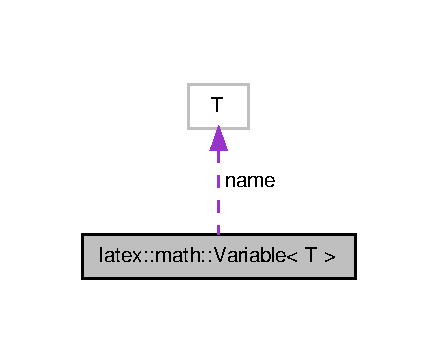
\includegraphics[width=210pt]{classlatex_1_1math_1_1Variable__coll__graph}
\end{center}
\end{figure}
\subsection*{\-Public \-Member \-Functions}
\begin{DoxyCompactItemize}
\item 
\hypertarget{classlatex_1_1math_1_1Variable_a2844e58e3a136631a4180811d6773f01}{{\bfseries \-Variable} (const \-T \&name)}\label{classlatex_1_1math_1_1Variable_a2844e58e3a136631a4180811d6773f01}

\item 
\hypertarget{classlatex_1_1math_1_1Variable_a3b9a17bd28ddfaf85c5634e6a8c7144d}{void {\bfseries solve} ()}\label{classlatex_1_1math_1_1Variable_a3b9a17bd28ddfaf85c5634e6a8c7144d}

\item 
\hypertarget{classlatex_1_1math_1_1Variable_adcd90cb19f6793a54b6571cc30d42e07}{std\-::string {\bfseries latex} () const }\label{classlatex_1_1math_1_1Variable_adcd90cb19f6793a54b6571cc30d42e07}

\end{DoxyCompactItemize}
\subsection*{\-Public \-Attributes}
\begin{DoxyCompactItemize}
\item 
\hypertarget{classlatex_1_1math_1_1Variable_a48cda4ab42456ea087dfe149653a1972}{\-T {\bfseries name}}\label{classlatex_1_1math_1_1Variable_a48cda4ab42456ea087dfe149653a1972}

\end{DoxyCompactItemize}
\subsection*{\-Friends}
\begin{DoxyCompactItemize}
\item 
\hypertarget{classlatex_1_1math_1_1Variable_a501b51eeedf7e93b817dc202b14a44a7}{std\-::ostream \& {\bfseries operator$<$$<$} (std\-::ostream \&os, const \hyperlink{classlatex_1_1math_1_1Variable}{\-Variable} \&var)}\label{classlatex_1_1math_1_1Variable_a501b51eeedf7e93b817dc202b14a44a7}

\end{DoxyCompactItemize}
\subsubsection*{template$<$typename T = std\-::string$>$ class latex\-::math\-::\-Variable$<$ T $>$}



\-The documentation for this class was generated from the following file\-:\begin{DoxyCompactItemize}
\item 
latex.\-hpp\end{DoxyCompactItemize}

\addcontentsline{toc}{part}{Index}
\printindex
\end{document}
